%% JAIR submission build (Volume 83+ ACM-based style, jair.cls wrapping acmart).
%% Generated from the reviewed manuscript; TMLR build preserved in main.tex.
\documentclass[manuscript, screen, review]{jair}

\setcopyright{cc}
\acmDOI{10.1613/jair.1.xxxxx}
\JAIRAE{To be assigned}
\JAIRTrack{}
\acmVolume{1}
\acmArticle{1}
\acmMonth{6}
\acmYear{2026}

%% --- Packages the manuscript needs that acmart does not already provide. ---
%% (acmart supplies amsmath, amssymb, graphicx, booktabs, xcolor, microtype,
%%  caption, hyperref, url -- do NOT re-load those.)
\usepackage{multirow}
\usepackage{subcaption}
\usepackage{algorithm}
\usepackage{algpseudocode}
\usepackage{enumitem}

%% --- Bibliography: biblatex + biber, acmauthoryear style (JAIR-required). ---
\RequirePackage[
  datamodel=acmdatamodel,
  style=acmauthoryear,
  backend=biber,
  giveninits=true,
  uniquename=init
  ]{biblatex}
\renewcommand*{\bibopenbracket}{(}
\renewcommand*{\bibclosebracket}{)}
\addbibresource{references.bib}

%% Map the manuscript's natbib-style citation commands onto biblatex.
%% (acmauthoryear already defines \citet.)
\providecommand{\citep}{\parencite}
\providecommand{\citealp}{\cite}

%% =========================================================================
%% Notation and number macros (carried over verbatim from the manuscript).
%% =========================================================================
% --- Notation macros (used throughout). -----------------------------------
\newcommand{\algoname}[1]{\textsc{#1}}
\newcommand{\iql}{\algoname{IQL}}
\newcommand{\vdn}{\algoname{VDN}}
\newcommand{\qmix}{\algoname{QMIX}}
\newcommand{\gnnqmix}{\algoname{GNN-QMIX}}
\newcommand{\coordgrid}{\textsc{CoordGrid}}
\newcommand{\Qtot}{Q_{\mathrm{tot}}}
\newcommand{\Qi}{Q_i}
\newcommand{\Vi}{V_i}
\newcommand{\Aagent}{\mathcal{A}}
\newcommand{\Sset}{\mathcal{S}}
\newcommand{\Oset}{\mathcal{O}}
\newcommand{\Nset}{\mathcal{N}}
\newcommand{\Egraph}{\mathcal{E}}
\newcommand{\Gtask}{\mathcal{G}}
\newcommand{\mlpqmix}{\algoname{MLP-QMIX}}
\newcommand{\gatqmix}{\algoname{GAT-QMIX}}
\newcommand{\dgnqmix}{\algoname{DGN-QMIX}}

% --- Phase 8 numbers (capacity control + long-horizon, n=10 seeds). -------
% Final values from the n=10 extension (seeds 0-9), ring graph, 150k steps.
% All Phase 8 prose references these macros, so numbers live in one place.
\newcommand{\PEsteps}{150{,}000}      % per-run env steps in Phase 8
\newcommand{\PEseeds}{10}             % seeds per cell in Phase 8
% N=4 ring final-window return (mean):
\newcommand{\PEqmixNfour}{83.0}
\newcommand{\PEmlpNfour}{83.4}
\newcommand{\PEgnnNfour}{72.8}
% N=8 ring final-window return (mean):
\newcommand{\PEqmixNeight}{164.9}
\newcommand{\PEmlpNeight}{164.9}
\newcommand{\PEgnnNeight}{78.3}
% Decisive gaps + stats (n=10):
\newcommand{\PEgraphGapNfour}{-10.6}  % GNN-QMIX minus MLP-QMIX, N=4
\newcommand{\PEgraphGapNeight}{-86.6} % GNN-QMIX minus MLP-QMIX, N=8
\newcommand{\PEgraphDNfour}{-3.2}     % Cohen's d, graph contrast, N=4
\newcommand{\PEgraphDNeight}{-3.9}    % Cohen's d, graph contrast, N=8
\newcommand{\PEcapGapNeight}{0.0}     % MLP-QMIX minus QMIX, N=8 (capacity; null)
\newcommand{\PEmwuP}{0.0002}          % Mann-Whitney p, decisive contrasts
\newcommand{\PEgnnSDNeight}{30.9}     % GNN-QMIX seed SD at N=8
\newcommand{\PEmlpSDNeight}{3.3}      % MLP-QMIX (matched control) seed SD at N=8
\newcommand{\PEqmixSDNeight}{9.2}     % QMIX seed SD at N=8
% --- Line-topology robustness (n=10, 150k steps; App. robustness table). --
% Same protocol as the ring cells, higher-diameter graph. Confirms the
% graph penalty / capacity null are not specific to the ring.
\newcommand{\PLqmixNfour}{62.4}
\newcommand{\PLmlpNfour}{63.0}
\newcommand{\PLgnnNfour}{52.9}
\newcommand{\PLqmixNeight}{143.0}
\newcommand{\PLmlpNeight}{144.2}
\newcommand{\PLgnnNeight}{78.5}
\newcommand{\PLgraphGapNfour}{-10.0}  % GNN-QMIX minus MLP-QMIX, N=4, line
\newcommand{\PLgraphGapNeight}{-65.8} % GNN-QMIX minus MLP-QMIX, N=8, line
\newcommand{\PLgnnSDNeight}{29.5}     % GNN-QMIX seed SD at N=8, line
\newcommand{\PLmlpSDNeight}{2.7}      % MLP-QMIX seed SD at N=8, line
% --- Phase 3: MPE simple_spread external validity (n=10, 150k steps). ------
% Final-window return (mean; less negative is better). Same 5 algos, same
% locked config / protocol as Phase 8 -- only the environment changes.
% k-NN coordination graph (k=2): at N=3 this is necessarily complete (each
% agent links to both others); N=6 is the genuinely sparse / larger case.
\newcommand{\PMqmixNthree}{-44.9}
\newcommand{\PMmlpNthree}{-44.3}
\newcommand{\PMgnnNthree}{-42.4}
\newcommand{\PMqmixNsix}{-74.3}
\newcommand{\PMmlpNsix}{-59.6}
\newcommand{\PMgnnNsix}{-80.4}
\newcommand{\PMgraphGapNthree}{+2.0}  % GNN-QMIX minus MLP-QMIX, N=3 (NS)
\newcommand{\PMgraphGapNsix}{-20.8}   % GNN-QMIX minus MLP-QMIX, N=6 (sig)
\newcommand{\PMcapGapNthree}{+0.6}    % MLP-QMIX minus QMIX, N=3 (NS)
\newcommand{\PMcapGapNsix}{+14.6}     % MLP-QMIX minus QMIX, N=6 (sig under MWU)
\newcommand{\PMgraphDNsix}{-1.46}     % Cohen's d, graph contrast, N=6
\newcommand{\PMcapDNsix}{+1.03}       % Cohen's d, capacity contrast, N=6
\newcommand{\PMgraphHolmNsix}{0.014}  % graph contrast, Holm over 3 decisive
\newcommand{\PMgraphMwuNsix}{0.009}   % graph contrast, Mann-Whitney
\newcommand{\PMcapMwuNsix}{0.045}     % capacity contrast, Mann-Whitney
\newcommand{\PMnetNsix}{-6.2}         % net GNN-QMIX minus QMIX, N=6 (NS, p=0.41)
% --- Phase 10: second GNN family (GAT-QMIX), n=10, 150k steps. ------------
% CoordGrid ring; the decisive contrast is GAT vs the no-graph MLP control.
\newcommand{\PGgatCGNfour}{75.6}      % GAT-QMIX final return, CoordGrid N=4 ring
\newcommand{\PGgatCGNeight}{110.1}    % GAT-QMIX final return, CoordGrid N=8 ring
\newcommand{\PGgatMlpNfour}{-7.8}     % GAT-QMIX - MLP-QMIX, N=4 (sig)
\newcommand{\PGgatMlpDNfour}{-2.0}    % Cohen d, GAT vs MLP, N=4
\newcommand{\PGgatMlpNeight}{-54.8}   % GAT-QMIX - MLP-QMIX, N=8 (sig)
\newcommand{\PGgatMlpDNeight}{-5.5}   % Cohen d, GAT vs MLP, N=8
\newcommand{\PGgatGnnNeight}{+31.8}   % GAT-QMIX - GNN-QMIX, N=8 (attention beats GCN)
\newcommand{\PGgatGnnDNeight}{+1.3}   % Cohen d, GAT vs GNN, N=8
\newcommand{\PGgatMpeNthree}{-8.1}    % GAT-QMIX - MLP-QMIX, MPE N=3 (MWU sig)
\newcommand{\PGgatMpeNsix}{-12.2}     % GAT-QMIX - MLP-QMIX, MPE N=6 (dir., ns)
% --- DGN-QMIX: multi-head dot-product attention (DGN/G2ANet mechanism). ----
\newcommand{\PGdgnCGNfour}{73.2}      % DGN-QMIX final return, CoordGrid N=4 ring
\newcommand{\PGdgnCGNeight}{131.4}    % DGN-QMIX final return, CoordGrid N=8 ring
\newcommand{\PGdgnMlpNfour}{-10.3}    % DGN-QMIX - MLP-QMIX, N=4 (sig)
\newcommand{\PGdgnMlpDNfour}{-4.5}    % Cohen d, DGN vs MLP, N=4
\newcommand{\PGdgnMlpNeight}{-33.5}   % DGN-QMIX - MLP-QMIX, N=8 (sig)
\newcommand{\PGdgnMlpDNeight}{-1.6}   % Cohen d, DGN vs MLP, N=8
\newcommand{\PGdgnMpeNthree}{+4.1}    % DGN-QMIX - MLP-QMIX, MPE N=3 (ns)
\newcommand{\PGdgnMpeNsix}{-9.1}      % DGN-QMIX - MLP-QMIX, MPE N=6 (ns)
% --- Phase 11: graph-penalty scaling on CoordGrid ring, n=10, 150k. -------
% Graph effect = GNN-QMIX - MLP-QMIX (negative); magnitude grows with N.
\newcommand{\PSgapNfour}{-10.6}       % (= Phase 8 N=4, for the trend)
\newcommand{\PSgapNeight}{-86.6}      % (= Phase 8 N=8)
\newcommand{\PSgapNtwelve}{-153.4}    % N=12
\newcommand{\PSgapNsixteen}{-267.4}   % N=16
\newcommand{\PSgnnNsixteen}{60.6}     % GNN-QMIX final return, N=16
\newcommand{\PSqmixNsixteen}{336.6}   % QMIX final return, N=16
\newcommand{\PSgnnFracNsixteen}{18}   % GNN as % of QMIX at N=16

% --- Stage C: the positive boundary (pair-routing under partial info). -----
% Structure-isolating arms on CoordGrid(pair_routing): SAME repaired GCN
% (residual + LayerNorm, L=2, width 64); only env.adjacency() differs.
%   gnn_true     = the task matching        (the right edges)
%   gnn_wrong    = a wrong matching, same 1-regular density
%   gnn_complete = all-to-all (most communication)
%   mlp          = no-comm parameter-matched control
% All Stage C prose references these macros; numbers come from
% results/phaseC/{summary,struct_verdict}_*.csv (>=12 seeds, 30k steps).
\newcommand{\gtrue}{\texttt{gnn\_true}}
\newcommand{\gwrong}{\texttt{gnn\_wrong}}
\newcommand{\gcomplete}{\texttt{gnn\_complete}}
\newcommand{\mlpc}{\texttt{mlp}}
\newcommand{\pairrouting}{\textsc{PairRouting}}
% Reference points on the N=6 pair-routing task (measured):
\newcommand{\SCfloor}{50}             % random / do-nothing return
\newcommand{\SCoracle}{149}           % full-information greedy oracle (~max 150)
% Headline cell: N=6, 3x3 grid, ego obs, 12 seeds, 30k steps.
\newcommand{\SCtrueN}{66.10}          % gnn_true final return
\newcommand{\SCtrueLo}{63.56}
\newcommand{\SCtrueHi}{68.65}
\newcommand{\SCwrong}{50.42}          % gnn_wrong
\newcommand{\SCwrongLo}{49.81}
\newcommand{\SCwrongHi}{51.02}
\newcommand{\SCcomplete}{50.94}       % gnn_complete (all-to-all)
\newcommand{\SCcompleteLo}{50.16}
\newcommand{\SCcompleteHi}{51.73}
\newcommand{\SCmlp}{49.85}            % mlp control
\newcommand{\SCmlpLo}{49.33}
\newcommand{\SCmlpHi}{50.38}
\newcommand{\SCfrac}{16}              % gnn_true as % of routing headroom (~50->149)
% Decisive (structure-isolating) contrasts, N=6:
\newcommand{\SCtwGap}{+15.7}          % gnn_true - gnn_wrong
\newcommand{\SCtwD}{5.4}              % Cohen's d
\newcommand{\SCtcGap}{+15.2}          % gnn_true - gnn_complete
\newcommand{\SCtcD}{5.1}
\newcommand{\SCtmGap}{+16.3}          % gnn_true - mlp (a-priori sanity)
\newcommand{\SCtmD}{5.6}
\newcommand{\SCpHolm}{<10^{-4}}       % Welch p_holm (all three; actual ~3.3e-8)
\newcommand{\SCsep}{61.5}             % min(gnn_true) across 12 seeds
\newcommand{\SCsepRivals}{52.6}       % max over all rival seeds
% N-robustness (gnn_true - mlp), significant at every N but NON-MONOTONE:
\newcommand{\SCnFourGap}{+11.8}
\newcommand{\SCnFourD}{3.3}
\newcommand{\SCnSixGap}{+16.3}
\newcommand{\SCnSixD}{5.6}
\newcommand{\SCnEightGap}{+16.4}
\newcommand{\SCnEightD}{3.0}
\newcommand{\SCnTenGap}{+11.0}
\newcommand{\SCnTenD}{1.6}
% Observability robustness (N=6, full obs): effect is LARGER.
\newcommand{\SCfullGap}{+22.6}        % gnn_true - mlp under full obs
\newcommand{\SCfullD}{5.4}
% Degree-2 topology (nbr_routing: ring / skip_ring / complete), N=6, 12 seeds:
\newcommand{\SCnbrTrue}{52.67}
\newcommand{\SCnbrWrong}{50.07}
\newcommand{\SCnbrComplete}{50.48}
\newcommand{\SCnbrMlp}{50.23}
\newcommand{\SCnbrTwGap}{+2.6}        % true - wrong
\newcommand{\SCnbrTwD}{1.7}
\newcommand{\SCnbrTcGap}{+2.2}        % true - complete
\newcommand{\SCnbrTcD}{1.4}
\newcommand{\SCnbrTmGap}{+2.4}        % true - mlp
\newcommand{\SCnbrTmD}{1.5}
\newcommand{\SCnbrPHolm}{0.005}       % all degree-2 contrasts p_holm < 0.005
\newcommand{\SCnbrShrink}{7}          % ~7x smaller than degree-1
% Attention arms (N=6, ego) -- STABILIZATION-MATCHED (residual+LayerNorm added
% to GAT/DGN), 12 seeds. Now cleanly identified (no stabilization confound).
\newcommand{\SCgatComplete}{50.19}    % gat_true's all-to-all sibling (floor)
\newcommand{\SCdgnComplete}{50.45}    % multi-head attention / all-to-all (floor)
\newcommand{\SCgatTrue}{67.03}        % attention / true matching: trains as well as GCN
\newcommand{\SCgatTrueGap}{+0.9}      % gat_true - gnn_true = +0.93 (n.s., p=0.64)
\newcommand{\SCgatTrueP}{0.64}        % Welch p, gat_true vs gnn_true (not significant)
\newcommand{\SCtrueGatCompGap}{+15.9} % gnn_true - gat_complete (floor contrast)
\newcommand{\SCtrueDgnCompGap}{+15.7} % gnn_true - dgn_complete (floor contrast)
\newcommand{\SCtrueAttCompD}{5.5}     % Cohen's d, gnn_true vs attention-over-all-to-all
% --- Stage D: out-of-harness replication in TokenMatch (no grid/movement). --
% Referential matching game: each agent must OUTPUT its partner's private
% token, routable only over the graph. SAME structure arms (only adjacency
% differs). N=6, K=5 tokens, 12 seeds. Numbers from STAGE_C_FINDINGS.md sec.7.
\newcommand{\tokenmatch}{\textsc{TokenMatch}}
\newcommand{\TMmax}{60}               % task maximum
\newcommand{\TMfloor}{12}             % random floor (~)
\newcommand{\TMmlp}{11.90}            % mlp (no comm)
\newcommand{\TMmlpLo}{11.67}
\newcommand{\TMmlpHi}{12.14}
\newcommand{\TMwrong}{12.03}          % gnn_wrong
\newcommand{\TMwrongLo}{11.78}
\newcommand{\TMwrongHi}{12.27}
\newcommand{\TMcomplete}{24.50}       % gnn_complete (all-to-all: PARTIAL routing)
\newcommand{\TMcompleteLo}{24.18}
\newcommand{\TMcompleteHi}{24.81}
\newcommand{\TMtrue}{57.59}           % gnn_true (near-solves: ~96% of max)
\newcommand{\TMtrueLo}{57.55}
\newcommand{\TMtrueHi}{57.63}
\newcommand{\TMfrac}{96}              % gnn_true as % of max (57.6/60)
\newcommand{\TMtwGap}{+45.6}          % gnn_true - gnn_wrong
\newcommand{\TMtcGap}{+33.1}          % gnn_true - gnn_complete
\newcommand{\TMtmGap}{+45.7}          % gnn_true - mlp

% --- Title block. ---------------------------------------------------------
\title{When Does Graph Structure Help in Multi-Agent\\
       Reinforcement Learning? A Controlled Boundary}

\begin{document}

\title[Graph Structure in Multi-Agent RL]{When Does Graph Structure Help in Multi-Agent Reinforcement Learning? A Controlled Boundary}

%% TODO(authors): JAIR is single-blind -- replace the placeholders below with the
%% full author list, affiliations, and ORCIDs before submission.
\author{Kasra Ghanavati}
\email{kasraghanavati@icloud.com}
\orcid{0000-0000-0000-0000}
\affiliation{%
  \institution{PLACEHOLDER -- institution}
  \city{PLACEHOLDER}
  \country{PLACEHOLDER}}
\renewcommand{\shortauthors}{Ghanavati}

\begin{abstract}
Graph neural network (GNN) value-factorisation methods are widely claimed
to outperform graph-free baselines in cooperative multi-agent
reinforcement learning (MARL) by exploiting relational inductive bias.
The conditions under which the claim holds are under-characterised: prior
work typically reports a single benchmark in a single graph regime,
conflating the contribution of the graph with that of added capacity,
and leaving the alignment between the GNN's receptive field and the task's
coordination structure unexamined. We close this gap with a controlled
empirical study on \coordgrid, a cooperative gridworld whose coordination
graph is itself the experimental variable. Holding the per-agent encoder,
state-conditioned mixer, optimiser, and exploration schedule fixed across
algorithms, we test pre-registered hypotheses on a structured graph
(H1), against a random graph of matched edge density (H2), and across
a GNN-depth $\times$ graph-diameter grid (H3), and we add a
parameter-matched no-graph control (\mlpqmix) that isolates the graph
from the extra capacity it brings.
The answer has two endpoints, and we identify both. \emph{Negative
endpoint.} When the task is full-information or reducible to a global
convention, \gnnqmix\ \emph{underperforms} the structurally simpler \qmix,
opposite to the prevailing claim, and the gap is \emph{identified}: against
\mlpqmix, which has byte-identical parameters but no graph aggregation,
\gnnqmix\ is significantly worse (Cohen's $d=\PEgraphDNeight$ at $N=8$;
Mann--Whitney $p=\PEmwuP$) while \mlpqmix\ matches \qmix, so the penalty is
the graph aggregation, not added capacity. It survives $5\times$ the
training budget (\PEsteps\ steps, \PEseeds\ seeds), \emph{destabilises}
learning, and grows with team size out to $N{=}16$. The same picture holds
on standard benchmarks: on MPE \texttt{simple\_spread} the penalty reappears
once a parameter-matched control decomposes it (the naive \gnnqmix-vs-\qmix\
comparison is null), and on Level-Based Foraging the graph is
neutral-to-harmful (significantly below \qmix\ at three agents; the
matched-control contrast is directional but not powered for significance at
$n{=}5$)---a regime where the graph is never significantly positive.
\emph{Positive endpoint.} On a constructed pair-routing task
in which each agent must reach its partner's \emph{private} goal (ego
observations), so the needed information is held by one specific other agent,
the task-matched graph beats all-to-all communication---which carries the
partner's information but must select it---at byte-identical parameters and
observations (Cohen's $d\approx5$; $+16$ return over a random floor of
${\sim}50$ at degree-1; Welch with Holm correction and Mann--Whitney
$p<10^{-4}$, complete seed-level separation at $n{=}12$); a density-matched
\emph{wrong} graph, which carries no partner information by construction,
floors alongside the no-graph control. On this task more communication did not
help (all-to-all floors); in a second task (\tokenmatch) all-to-all manages
only weak partial routing ($+12$) yet still falls $-33$ below the matched
graph---so it is the \emph{right} communication, not more of it, that matters,
and the advantage is graph \emph{structure},
not the channel or the capacity, and is not recovered by aggregator
expressiveness alone: neither a fixed mean-aggregator nor a stabilisation-matched
\emph{learned} attention head---which could in principle up-weight the
partner---recovers the partner's signal from all-to-all within our training
budget, while given the right graph a more expressive aggregator trains at
least as well (an exploratory, not pre-registered, $+5.4$ for multi-head
attention over the GCN)---so expressiveness amplifies structure but cannot
substitute for it. The effect is significant at every
team size $N{=}4$--$10$ but \emph{non-monotone} (it does not grow as a
dose-response), is robust to full observability, and persists at degree-2
(genuine topology) though about $\SCnbrShrink\times$ smaller at the
pre-registered 30k budget (exploratory longer-budget runs suggest the gap
grows, so this attenuation factor is an upper bound). It replicates
out of harness in a non-spatial token-matching game, so it is not a gridworld
artefact. We state scope plainly: this is a constructed-task
existence/boundary result---replication on a standard third-party benchmark is
still future work, and this positive endpoint is a mechanism/existence result
rather than a turnkey recipe. The practical rule, stated conditionally: add a
coordination graph, and route along task-relevant edges rather than all-to-all,
only when agents must act on information held by specific others they cannot
observe \emph{and} the coordination topology is known or reliably estimable
(our controls show the obvious fallbacks---a wrong graph, or all-to-all---do not
recover the benefit). We
release the harness, configs, and plotting code as supplementary material
(Appendix~\ref{app:repro}).
\end{abstract}

\maketitle


% =========================================================================
\section{Introduction}
\label{sec:intro}

Cooperative multi-agent reinforcement learning (MARL) underlies progress on
team coordination problems from traffic signal control to multi-robot
manipulation. Value-decomposition methods, in which a joint team Q-value
$\Qtot$ is factorised into per-agent utilities $\Qi$ for centralised
training and decentralised execution, have emerged as a workhorse:
\vdn~\citep{sunehag_2018_vdn} factorises $\Qtot$ as a sum, \qmix
\citep{rashid_2018_qmix,rashid_2020_qmix_jmlr} as a monotonic mixture, and
several recent methods extend the mixer with graph neural networks (GNNs)
over an externally specified or learned coordination graph
\citep{jiang_2020_dgn,liu_2020_g2anet,boehmer_2020_dcg,
       naderializadeh_2020_graphmix}.

The intuition for graph-based MARL is straightforward: when agents form
a coordination \emph{structure}, a model whose architecture mirrors that
structure should generalise better and converge faster. This intuition
is widely cited as motivation in the literature, yet the conditions
under which it actually holds are surprisingly under-tested. Three
specific gaps motivate the present study:

\begin{enumerate}[leftmargin=*,itemsep=0pt,topsep=2pt]
  \item \textbf{Graph regime is rarely varied.} Most empirical comparisons
        fix one environment with one (often implicit) coordination graph,
        leaving open whether observed gains transfer to other graphs:
        sparse vs.\ dense, structured vs.\ random.
  \item \textbf{Capacity is rarely controlled.} Adding a GNN adds
        parameters and depth as well as relational structure. Without a
        controlled comparison it is unclear whether the win comes from the
        graph or from the extra capacity.
  \item \textbf{Receptive-field alignment is rarely studied.} A GNN of
        depth $L$ propagates information across paths of length up to $L$.
        It is intuitive that $L$ should grow with the graph's diameter. The
        general depth/long-range trade-off is well studied for GNNs
        (over-squashing on long-range tasks~\citep{alon_2021_oversquashing},
        over-smoothing with depth~\citep{li_2018_oversmoothing}), but we
        found no empirical study of receptive-field-versus-diameter alignment
        for a GNN inserted into a value-factorisation mixer (CTDE),
        specifically in the cooperative MARL setting.
\end{enumerate}

\paragraph{A two-endpoint answer.} The title question is not a yes/no, and we
answer it by locating \emph{both} endpoints of a boundary under one
controlled harness. At one endpoint---full-information or
convention-reducible tasks, where any agent could in principle infer what it
needs without the graph---a graph-conditioned mixer is neutral to actively
harmful, and a capacity-matched control pins the harm on the graph
aggregation itself rather than on added parameters. At the other endpoint we
\emph{construct} the regime the first leaves unexplored: a task in which an
agent must act on private information held by one specific partner it cannot
observe, so the coordination graph is the only path for that information.
There, message passing helps---but only when the communication topology
matches the task's coordination edges; pointing the same channel at the
wrong neighbours leaves it at the no-communication floor, and broadcasting to
everyone does at most weak, task-incidental routing far below the task-matched
graph. The two
endpoints \emph{coexist}: the positive result completes the negative one
into a single ``when does it help'' statement rather than overturning it.

\paragraph{Contributions.} This paper makes the following contributions.

\begin{enumerate}[leftmargin=*,itemsep=0pt,topsep=2pt]
  \item We introduce \coordgrid\ (Figure~\ref{fig:overview}A), a cooperative
        gridworld whose coordination graph is a tunable knob (ring, line,
        complete graph, lattice, Erd\H{o}s--R\'enyi). The reward is defined
        edge-wise over this graph, so the graph is literally the
        coordination structure rather than a heuristic over a fixed task.
  \item We implement \iql, \vdn, \qmix, and \gnnqmix\ in a single harness
        with shared encoder, mixer, optimiser, and exploration schedule
        (Figure~\ref{fig:overview}B), so the only difference between
        \gnnqmix\ and \qmix\ is the GNN. To isolate the graph from the
        capacity it adds (Gap~2) we include \mlpqmix, a parameter-matched
        no-graph control (byte-identical parameter count, no neighbour
        aggregation); and \gatqmix, a graph-\emph{attention} variant that
        tests whether the result is specific to the fixed GCN.
  \item We pre-register three falsifiable hypotheses
        (Section~\ref{sec:hypotheses}) and test them with a pilot,
        a graph-regime sweep, and a depth $\times$ diameter ablation
        (Sections~\ref{sec:results:pilot}--\ref{sec:results:ablation}).
  \item \textbf{The negative endpoint.} In full-information /
        convention-reducible settings the prevailing positive picture of
        graph-based MARL does not survive a controlled comparison:
        \gnnqmix\ is bested by \qmix\ in both mean return and seed-level
        variance, even on an edge-defined-reward task whose observations
        (under the non-ego obs mode used here) already expose neighbour
        displacements, so message passing is at best redundant. The
        non-trivial finding is not a surprising failure but the
        capacity-matched \emph{identification} of the cause. The capacity control
        (\S\ref{sec:results:capacity}) \emph{identifies} the cause (the
        no-graph \mlpqmix\ matches \qmix\ while \gnnqmix\ falls far below
        both, so the penalty is the graph aggregation, not the added
        parameters) and shows it survives a $5\times$ longer training budget
        at $n{=}\PEseeds$ seeds (ruling out undertraining), and that the
        \emph{negative} penalty grows monotonically with team size out to
        $N{=}16$ (distinct from the \emph{positive} structure effect of
        contribution~5, which is significant at every $N$ but non-monotone).
        On MPE \texttt{simple\_spread} the penalty reappears under the
        capacity decomposition (the naive \gnnqmix-vs-\qmix\ comparison is
        null at $N{=}6$; \S\ref{sec:results:mpe}); on \coordgrid\ it persists
        when the GCN is replaced by graph attention
        (\S\ref{sec:results:capacity}), which on MPE narrows but is not
        significant.
  \item \textbf{The positive endpoint} (\S\ref{sec:results:structure}). We
        pre-register and run a constructed pair-routing task in which each
        agent must reach a partner's \emph{private} goal, so the graph is the
        only path for task-structured information. There the task-matched
        graph beats all-to-all communication---which carries the partner's
        information but must select it---at byte-identical parameters and
        observations ($d\approx5$ at degree-1; Welch/Holm and Mann--Whitney
        $p<10^{-4}$); a density-matched wrong graph, which carries no partner
        information by construction, floors alongside the no-graph control.
        More communication did not help, the \emph{right} communication did.
        The advantage is the structure, not the channel or the capacity, and is
        not recovered by expressiveness alone: neither the fixed mean-aggregator
        nor a stabilisation-matched learned attention head recovers the signal
        from all-to-all within budget, while given the right graph a more
        expressive aggregator trains at least as well (an exploratory,
        not pre-registered, multi-head-attention $+5.4$ over the GCN).
        The effect is significant at every $N{=}4$--$10$ (but
        non-monotone), robust to observability, survives at degree-2 about
        $\SCnbrShrink\times$ smaller at the 30k budget (an upper bound on the
        attenuation; longer-budget runs suggest a smaller gap), and replicates
        out of harness in a non-spatial token-matching game (not a gridworld
        artefact).
  \item The depth--diameter alignment heuristic (H3) is falsified in favour
        of a sharper practitioner rule (\S\ref{sec:results:ablation}): a
        hard over-depth cliff means GCN depth should not exceed two in
        small-team CTDE settings.
\end{enumerate}

\begin{figure}[t]
  \centering
  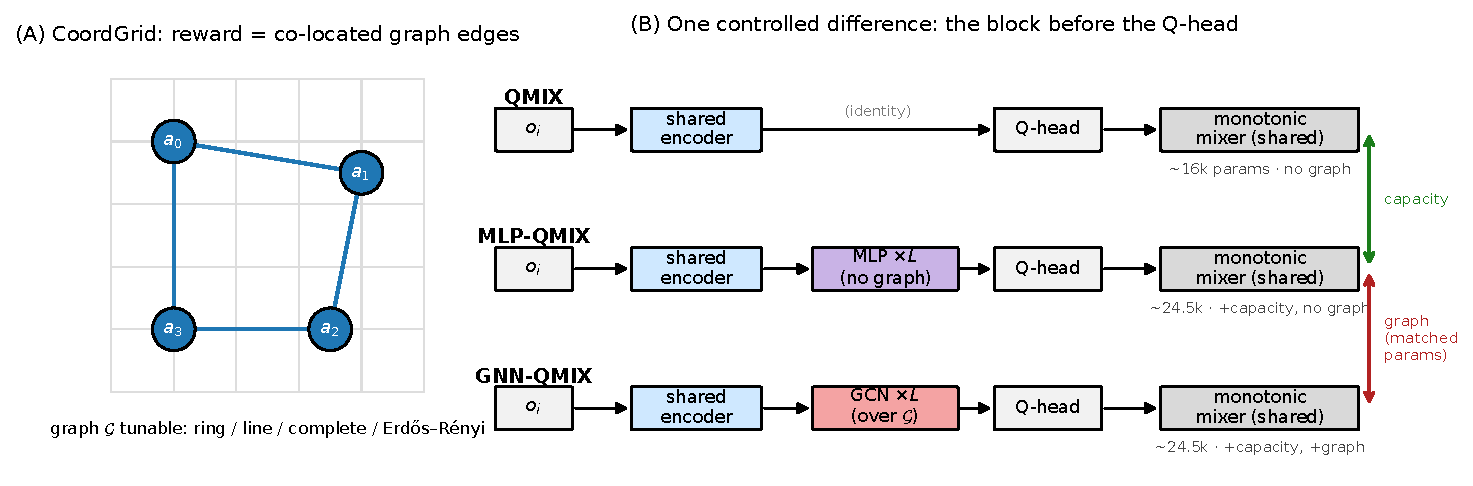
\includegraphics[width=\textwidth]{figures/fig1_overview.pdf}
  \caption{\textbf{Setup and controlled comparison.} (A) \coordgrid:
  agents act on a grid wired by a \emph{tunable} coordination graph
  $\Gtask$; the reward is the number of graph edges whose endpoints are
  co-located, so the graph \emph{is} the coordination structure. (B) All
  algorithms share an identical per-agent encoder and monotonic mixer and
  differ only in the block inserted before the Q-head. \qmix\ inserts
  nothing; \gnnqmix\ inserts an $L$-layer GCN over $\Gtask$; \mlpqmix\
  inserts an $L$-layer MLP of \emph{identical parameter count} but no
  graph. \gnnqmix\ vs.\ \mlpqmix\ isolates the \emph{graph} (matched
  parameters); \mlpqmix\ vs.\ \qmix\ isolates the \emph{capacity}.}
  \label{fig:overview}
\end{figure}

% =========================================================================
\section{Background and Notation}
\label{sec:background}

\paragraph{Decentralised partially observable Markov decision process
(Dec-POMDP).} A cooperative MARL task is a tuple
$\langle \Nset, \Sset, \{\Aagent_i\}, P, R, \{\Oset_i\}, \{O_i\}, \gamma
\rangle$, where $\Nset = \{1,\dots,N\}$ are agents, $\Sset$ the global
state, $\Aagent_i$ the discrete action set of agent $i$,
$P(s' \mid s, \mathbf{a})$ the transition kernel, $R(s, \mathbf{a})$ a
shared scalar reward, and $O_i(s) \in \Oset_i$ the local observation
function. Agents share the discount $\gamma$ and select actions from
$\Oset_i$; centralised training (with access to $s$) is permitted while
execution is decentralised \citep{oliehoek_2016_decpomdp}.

\paragraph{Centralised training with decentralised execution (CTDE) and
value factorisation.} Value factorisation methods learn per-agent
utilities $\Qi(o_i, a_i)$ and a centralised mixer that combines them into
$\Qtot$:
\[
  \Qtot(s, \mathbf{a}) = f_{\text{mix}}\bigl(\Qi(o_i, a_i)\,;\,s\bigr),
\]
trained against a Bellman target on the team reward. The decentralised
greedy policy $\pi_i(o_i) = \arg\max_{a_i} \Qi(o_i, a_i)$ recovers the
joint greedy action when $f_{\text{mix}}$ satisfies the Individual-Global-Max
(IGM) condition \citep{son_2019_qtran}.

\paragraph{Coordination graph.} We define a coordination graph
$\Gtask = (\Nset, \Egraph)$ over the agents. \coordgrid\ (Section
\ref{sec:env}) ties the per-step reward to $\Egraph$ directly: only
\emph{edges} contribute reward, so the coordination structure is not a
heuristic about the environment but a literal description of it.
\gnnqmix\ takes $\Gtask$ as side information; \iql/\vdn/\qmix\ do not.

% =========================================================================
\section{Related Work}
\label{sec:related}

\paragraph{Value-decomposition MARL.} \iql~\citep{tan_1993_marl} ignores
agent interaction and trains independent Q-learners on the shared reward,
which is biased but a useful no-coordination baseline. \vdn
\citep{sunehag_2018_vdn} sums per-agent utilities. \qmix
\citep{rashid_2018_qmix,rashid_2020_qmix_jmlr} learns a monotonic state-conditioned
mixer via a hypernetwork, enforcing $\partial \Qtot / \partial \Qi \geq 0$
so decentralised greedy execution is consistent with the centralised
argmax. \algoname{QTRAN} \citep{son_2019_qtran} and \algoname{MAVEN}
\citep{mahajan_2019_maven} relax or extend the monotonicity assumption;
\algoname{QPLEX} \citep{wang_2021_qplex} reformulates it through a
duplex dueling architecture. Beyond value-factorisation,
\algoname{MAPPO} \citep{yu_2022_mappo} shows that vanilla PPO with
centralised critics is a surprisingly strong cooperative baseline; we
restrict scope to value-decomposition methods to keep the architectural
contrast with \gnnqmix\ clean.

\paragraph{Learned and pre-specified inter-agent communication.}
Pre-dating the graph-MARL literature, \algoname{RIAL/DIAL}
\citep{foerster_2016_rial_dial} and \algoname{CommNet}
\citep{sukhbaatar_2016_commnet} learn pairwise or all-to-all
communication channels between agents. These methods can be viewed as
implicitly learning a (typically dense) coordination graph rather than
taking one as input. We exclude them from the experimental comparison
because they confound the question we want to answer (does \emph{a given}
graph help?) with the orthogonal question (can the agents learn a useful
graph?).

\paragraph{Graph-based MARL.} \algoname{DGN} \citep{jiang_2020_dgn} applies
graph convolution over a $k$-NN agent graph, evaluated on both discrete
and continuous cooperative tasks.
\algoname{G2ANet} \citep{liu_2020_g2anet} uses attention to abstract a
game graph. \algoname{Deep Coordination Graphs}
\citep{boehmer_2020_dcg} factor $\Qtot$ over a hyperedge structure.
\algoname{GraphMIX} \citep{naderializadeh_2020_graphmix} interleaves a GNN
with a QMIX-style monotonic mixer, closest in spirit to the
\gnnqmix\ baseline we evaluate here. Our \gnnqmix\ is a deliberately
\emph{minimal} instantiation of this GraphMIX-style ``GNN + monotonic mixer''
family rather than a re-implementation of GraphMIX's full pipeline: it
takes the coordination graph as an \emph{external input} (rather than learning
it), inserts a fixed-GCN encoder \emph{before} an otherwise-unchanged QMIX
mixer, and leaves the mixer untouched---so the GCN is the only structural
variable, which is what makes the wrong-graph/all-to-all contrasts clean
isolators (and is not intended as a strawman: it is chosen to isolate the GCN,
not to weaken the baseline).

It is useful to separate these methods along a \emph{fixed-vs-learned-graph}
axis, because that axis is exactly what our controls exploit. At one end,
\algoname{DCG} and our \gnnqmix/GraphMIX\ take the interaction graph as an
explicit input. \algoname{DGN} sits between: its graph is a \emph{fixed}
$k$-NN-by-proximity rule, recomputed as agents move but not learned. At the
other end the graph is \emph{inferred}---\algoname{G2ANet}'s learned attention
graph, \algoname{DICG} \citep{li_2021_dicg}, which infers a dynamic
coordination graph for a GNN, and the context-aware sparse coordination graphs
of \algoname{CASEC} \citep{wang_2022_casec} and \algoname{Non-Linear
Coordination Graphs} \citep{kang_2022_nonlinearcg}. Of these, \algoname{CASEC}
is the closest qualitative precedent for our headline: it argues and shows that
\emph{sparse} coordination graphs outperform dense/static ones. We credit that
``sparse beats complete'' is already established; our delta is the controlled
\emph{attribution}. CASEC (and the learned-graph line generally) \emph{learns}
the sparse topology and measures task return, so its gain entangles sparsity,
learned selection, and capacity. We instead \emph{fix} the topology and contrast
a task-matched graph against a \emph{density-matched wrong} graph and all-to-all
at byte-identical parameters and observations---the density-matched wrong graph
is what isolates the effect to \emph{which} edges rather than to sparsity or to
the act of learning a graph. Even \algoname{DCG}, the closest fixed-graph
relative, defines payoffs over \emph{given} hyperedges but never runs a
wrong-graph control, so it cannot separate topology-correctness from the mere
presence of a graph. More generally these methods combine three design choices
(a graph, a message-passing mechanism, and a value mixer) in ways that make it
difficult to attribute observed gains to any single component; our study
isolates the GNN encoder by inserting it into an otherwise-identical \qmix\
architecture.

\paragraph{Communication under partial observability.} A parallel line of
work motivates inter-agent message passing precisely by partial
observability: when an agent cannot see what it needs, a learned channel can
carry it. \algoname{CommNet} \citep{sukhbaatar_2016_commnet} and
\algoname{DIAL} \citep{foerster_2016_rial_dial} learn such channels;
\algoname{DGN} \citep{jiang_2020_dgn} and \algoname{G2ANet}
\citep{liu_2020_g2anet} make the channel graph-structured (a fixed $k$-NN
graph and a learned attention graph, respectively). A closely related line
argues specifically that \emph{targeted} communication beats one-size-fits-all
broadcast: \algoname{TarMAC} \citep{das_2019_tarmac} learns signature-based
targeted messages, \algoname{IC3Net} \citep{singh_2019_ic3net} learns
\emph{when} to communicate, and \algoname{ATOC} \citep{jiang_2018_atoc} learns
an attentional communication group. This qualitatively anticipates our
finding that all-to-all is worse than the right targeted edges---but those
works \emph{learn} the targeting and run no density-matched wrong-graph or
parameter-matched no-graph control. We revisit this in
\S\ref{sec:structure:attention}: a learned attention head over all-to-all does
not recover the matched-graph advantage \emph{within our training budget},
which is consistent with---not contradictory to---TarMAC/ATOC succeeding, since
those methods invest substantial training in learning to target, and is not a
claim that attention cannot learn the targeting in principle. Our delta is distinct and complementary:
we \emph{fix} the topology and contrast a task-matched graph against a
density-matched wrong graph and all-to-all at byte-identical parameters,
isolating the contribution of \emph{structure} from that of the channel and of
the learned routing---a control these works do not run.
The positive endpoint we
identify sits squarely in this regime---private information that no agent can
observe locally---and is what reconciles it with our negative result: a
coordination graph earns its keep exactly when the task makes some agent's
information unavailable to the others, and not in the full-information
settings where prior controlled comparisons (and ours) find it inert. Where
these methods entangle ``does \emph{a} graph help?'' with ``can the agents
\emph{learn} a useful graph?'', we hold the graph fixed and vary only its
\emph{topology} relative to the task, which isolates the contribution of
structure from that of the channel.

\paragraph{Foundational GNNs.} We use a textbook graph convolutional
network~\citep{kipf_2017_gcn}; \citet{velickovic_2018_gat} and
\citet{xu_2019_gin} characterise alternatives.
\citet{battaglia_2018_gn} surveys the broader graph-network family.

\paragraph{Evaluation methodology.} Our protocol follows the recommendations
of \citet{henderson_2018_drlmatters} and \citet{agarwal_2021_precipice}:
multiple seeds, confidence intervals, an explicit sample-efficiency metric,
and Holm-corrected pairwise tests in place of $p<0.05$ readings off a
forest plot. We additionally report effect sizes (mean differences) so
readers do not have to infer them from CI overlap. Controlled comparisons of
value decomposition versus independent learning already exist:
\citet{papoudakis_2021_benchmarking} benchmark tuned IQL/VDN/QMIX across
MPE/LBF/SMAC and find independent learning \emph{competitive} on the
fully-observable MPE/LBF tasks while value decomposition wins where
coordination is genuinely required---squarely the territory of our negative
endpoint. They do not, however, include a graph-conditioned mixer or a
parameter-matched no-graph control; our contribution is to isolate the graph
\emph{aggregation} itself and attribute the penalty to it.

\paragraph{Benchmarks.} The Multi-agent Particle Environment
\citep{lowe_2017_maddpg} and PettingZoo \citep{terry_2021_pettingzoo}
provide canonical cooperative tasks; \algoname{SMAC}
\citep{samvelyan_2019_smac} is a heavier StarCraft micro-management
benchmark. We use \coordgrid\ as the primary test bed because it lets us
\emph{set} the coordination graph rather than infer it, and report a
restricted MPE replication in Section~\ref{sec:results:mpe}.

% =========================================================================
\section{Hypotheses}
\label{sec:hypotheses}

We test three pre-registered hypotheses:

\begin{description}[leftmargin=4em,style=nextline]
  \item[\textbf{H1 (structure beats no-structure):}]
    On a cooperative task whose reward is graph-edge-defined, \gnnqmix
    achieves a higher final return and crosses a fixed performance
    threshold sooner than \iql, \vdn, and \qmix\ when the underlying
    coordination graph is sparse and structured.
  \item[\textbf{H2 (structure $>$ matched-density random):}]
    The advantage of \gnnqmix\ over \qmix\ is larger on a structured
    graph (ring) than on an Erd\H{o}s--R\'enyi graph of the same edge
    density. This rules out the explanation that GNN-QMIX wins simply by
    having more inputs.
  \item[\textbf{H3 (depth--diameter inverted-U):}]
    Final return as a function of GNN depth $L$ peaks near $L \approx d$,
    where $d$ is the graph diameter, and degrades when $L$ is either
    substantially smaller (insufficient receptive field) or substantially
    larger (over-squashing, optimisation noise). \emph{Falsifiability
    criterion (pre-registered):} for each diameter $d$ tested, we declare
    a per-row match if (a) the mean depth-return curve is non-flat
    (relative range $(\max - \min)/\max \ge 0.10$), and (b) $|L^* - d|
    \le 1$ where $L^*$ is the empirical argmax depth. We declare the
    family-level H3 confirmed if at least $\lceil 2n/3 \rceil$ of the $n$
    tested diameters pass the per-row criterion.
\end{description}

% =========================================================================
\section{Experimental Design}
\label{sec:design}

\subsection{The \coordgrid\ environment}
\label{sec:env}

\coordgrid\ is a cooperative gridworld parameterised by the team size $N$,
the grid side $G$, the episode length $T$, and a coordination graph
$\Gtask$. The grid is toroidal. Each agent occupies a cell and chooses one
of five actions per step: stay, up, down, left, right. The reward at step
$t$ is
\[
  r_t \;=\; \sum_{(i,j) \in \Egraph} \mathbf{1}\bigl[p_i^{(t)} = p_j^{(t)}\bigr],
\]
where $p_i^{(t)}$ is agent $i$'s grid position at $t$. Reward is therefore
the count of \emph{graph edges} whose endpoints are co-located. Agents not
linked by an edge have no reason to coordinate spatially: the graph is
literally the coordination structure. Each agent observes its own
normalised position, the relative displacement to each of its graph
neighbours (zero-padded to a fixed slot count), and an agent-id one-hot.
The global state used by the mixer is the concatenation of all agents'
normalised positions.

\paragraph{Tunable graph regimes.} The implementation supports five graph
families: \texttt{complete} ($d=1$), \texttt{ring} ($d=\lfloor N/2 \rfloor$),
\texttt{line} ($d = N-1$), \texttt{grid2d} ($d = 2(\sqrt N - 1)$), and
\texttt{erdos\_renyi} (random $G(N, p)$ resampled per episode). The
diameter range $\{1, 2, 3, 4\}$ used in our ablation is achieved by
combining \texttt{complete} ($d=1$), \texttt{ring} on $N=4$ ($d=2$),
\texttt{line} on $N=4$ ($d=3$), and \texttt{line} on $N=5$ ($d=4$).

\subsection{Algorithms}
\label{sec:algos}

The five core algorithms below (\iql, \vdn, \qmix, \gnnqmix, and the
\mlpqmix\ control; a sixth, the graph-attention variant \gatqmix, is
introduced for the robustness check in \S\ref{sec:results:capacity})
share a per-agent Q-network, an MLP of the form
$\Aagent_i \mapsto \mathrm{ReLU}(\mathrm{Linear}_{64})
\rightarrow \mathrm{ReLU}(\mathrm{Linear}_{64})
\rightarrow \mathrm{Linear}_{|\Aagent_i|}$ with parameters shared across
agents and an agent-id one-hot appended to the observation. They share a
$5\times 10^{-4}$ Adam optimiser, $\gamma = 0.99$, replay capacity $5\times10^4$,
batch size 32, target hard updates every 200 gradient steps, Huber loss
with Double-DQN targets \citep{vanhasselt_2016_doubledqn}, and gradient norm
clipping at 10.

\begin{itemize}[leftmargin=*,itemsep=0pt,topsep=2pt]
  \item \iql: per-agent TD on the shared reward, no mixer.
  \item \vdn: $\Qtot = \sum_i \Qi(o_i, a_i)$.
  \item \qmix: $\Qtot = f_{\text{mix}}(s)(\Qi)$ where $f_{\text{mix}}$ is the
        standard hypernet mixer with absolute-value weights producing
        non-negative monotonicity, embedding dimension 32.
  \item \gnnqmix: per-agent encoders feed an $L$-layer GCN over the
        coordination graph $\Gtask$ before the Q heads, with $L=2$,
        hidden dimension 64. The mixer is \emph{identical} to \qmix; the
        GCN is the only structural change.
  \item \mlpqmix\ (parameter-matched no-graph control): identical to
        \gnnqmix\ in every respect except that the $L$-layer GCN is
        replaced by an $L$-layer MLP of the same per-layer shape, i.e.\ the neighbour-aggregation step $\tilde A H$ is removed,
        leaving $\mathrm{ReLU}(HW)$. \mlpqmix\ has a byte-identical
        parameter count to \gnnqmix\ at matched $(L, \text{width})$, so
        the only difference between the two is whether information
        crosses the coordination graph.
\end{itemize}

\paragraph{Why this matters: isolating graph from capacity.} The mixer,
optimiser, exploration schedule and per-agent encoder \emph{stem} are
identical across \qmix, \gnnqmix, and \mlpqmix. \gnnqmix\ inserts an
$L$-layer GCN of width 64 between the encoder and the Q head, adding
$L \cdot (64^2 + 64) \approx 4.2\,L$ thousand parameters that \qmix\ does
not have (e.g.\ $\sim 8.3$k at $L=2$, against $\sim 16$k for \qmix). A
comparison of \gnnqmix\ against \qmix\ alone therefore confounds two
explanations: the relational inductive bias of the \emph{graph}, or the
extra \emph{capacity}. \mlpqmix\ removes the confound by construction: it
carries exactly the same extra parameters but no graph. This yields a
three-way decomposition (verified to identical parameter counts in
Section~\ref{sec:results:capacity}): \qmix\ (no capacity, no graph),
\mlpqmix\ (capacity, no graph), \gnnqmix\ (capacity and graph). The
fully-identified test of ``does the graph help?'' is \gnnqmix\ vs.\
\mlpqmix\ at matched capacity; \mlpqmix\ vs.\ \qmix\ separately measures
whether the capacity alone matters. The depth-vs-diameter ablation
(Section~\ref{sec:results:ablation}, H3) additionally isolates depth
effects within \gnnqmix.

The full shared training loop (CTDE, off-policy, Double-DQN; identical
across algorithms modulo the \iql\ per-agent loss) is given as
Algorithm~\ref{alg:train} in Appendix~\ref{app:trainloop}.

\subsection{Evaluation protocol}
\label{sec:protocol}

Each run trains for a fixed number of environment steps and logs one CSV
row per episode (return, length, $\epsilon$, mean loss, gradient norm,
wall-clock). We report two metrics:

\begin{enumerate}[leftmargin=*,itemsep=0pt,topsep=2pt]
  \item \textbf{Final-window return}: mean return over the last 10\% of
        episodes of a run. This is a coarse capacity measure.
  \item \textbf{Episodes to 80\% of own final}: the first episode at
        which the 25-episode rolling mean reaches 80\% of that run's own
        final-window mean. This per-run \emph{self-threshold} is panel-
        invariant (adding or removing an algorithm does not change any
        other algorithm's number) and isolates ``how quickly does this
        configuration converge to its plateau'' from ``how high is its
        plateau,'' which the first metric already captures.
\end{enumerate}

Across-seed aggregates use the sample mean and the Student-$t$ 95\%
confidence interval. Pairwise algorithm comparisons use Welch's two-sample
$t$-test as the primary and Mann--Whitney $U$ as a non-parametric
robustness check, with Holm--Bonferroni step-down correction. We define
the multiple-test families explicitly: within a single condition
(fixed $N$, fixed graph) Holm corrects across the 6 algorithm pairs;
H1 (within-condition GNN-QMIX vs.\ QMIX) is one one-sided test per
condition and is not corrected within H1; H2 (interaction across
graph regimes) is a single one-sample $t$ on the per-seed
difference-of-differences $\Delta_{\text{ring}} - \Delta_{\text{ER}}$
against zero and is therefore uncorrected. Confidence intervals use the
Student-$t$ 95\% interval across the $10$ seeds run per condition; we report
effect sizes (mean differences) alongside $p$-values so readers do not have to
back-fit power from CI overlap. Number of seeds
and step budget per phase are listed in Table~\ref{tab:budget};
deviations from the originally pre-registered budget were forced by
compute constraints and are noted explicitly.

% =========================================================================
\section{Results}
\label{sec:results}

\subsection{Phase 1: Pilot}
\label{sec:results:pilot}

\textbf{Setup.} 4 agents, ring graph (diameter $d=2$), 10 seeds, $5 \times 10^4$
environment steps per run. This phase is a harness sanity check: per
\texttt{docs/PHASES.md}, the acceptance criterion is that the coordinated
baselines (\vdn, \qmix) clearly outperform \iql\ on a task with obvious
coordination demand, and \gnnqmix\ runs to completion.

\textbf{Findings.} Figure~\ref{fig:phase1_curves} and
Table~\ref{tab:phase1_summary} show the per-algorithm learning curves and
final-window returns. Three results:
\begin{enumerate}[leftmargin=*,itemsep=0pt,topsep=2pt]
  \item The harness reproduces the expected ordering of coordinated over
        independent learning: \qmix\ (mean $84.02$, 95\% CI
        $[83.41, 84.62]$) $>$ \vdn\ (mean $66.02$, CI $[62.57, 69.48]$) $>$
        \iql\ (mean $34.62$, CI $[32.61, 36.64]$).\footnote{\vdn\ and \gnnqmix\
        round to the same $66.02$ at two decimals ($66.023$ and $66.015$
        respectively; Table~\ref{tab:phase1_summary}); this is a coincidence of
        two independent runs, not a duplicated row---their CIs differ markedly
        ($[62.57, 69.48]$ vs.\ $[57.11, 74.92]$).} The \iql\ vs.\ \vdn\ gap
        is Holm-significant ($p_{\text{Holm}} < 0.001$) and the \iql\
        vs.\ \qmix\ gap strongly so ($p_{\text{Holm}} < 0.001$). The
        Phase-0 acceptance criterion is met.
  \item \gnnqmix\ is markedly \emph{worse} than \qmix\ on this condition
        (mean $66.02$ vs.\ $84.02$), and the gap is not attributable to
        capacity overhead (\gnnqmix\ has the extra GCN parameters; if
        anything, that would predict a small \emph{advantage} due to
        added expressiveness). Instead, \gnnqmix\ exhibits elevated
        seed-level variance: its $95\%$ CI spans $[57.11, 74.92]$, more than
        an order of magnitude wider than \qmix's $[83.41, 84.62]$, with the
        weakest seeds stalling in the low-return regime of \iql\
        (Figure~\ref{fig:phase1_curves}).
  \item This finding is the first sign that ``does graph structure
        help?'' is not a simple yes/no. On the easy case (small team,
        small diameter, abundant coordination signal), the simpler
        \qmix\ mixer is both more accurate and more stable. The
        remainder of the paper asks under what conditions the extra
        graph machinery in \gnnqmix\ does pay for itself.
\end{enumerate}

% Phase 1 pilot figure (fig:phase1_curves) and summary table
% (tab:phase1_summary) are collected in Appendix~\ref{app:fulltables} to
% keep the main-body figure budget for the headline results.


\subsection{Phase 2: Scale and graph regime (H1, H2)}
\label{sec:results:scale}

\textbf{Setup.} $N \in \{4, 8\} \times \{\text{ring}, \text{Erd\H{o}s--R\'enyi
with matched density}\} \times 4$ algorithms $\times$ 10 seeds at
$3\times 10^4$ env steps per run. We shorten the pre-registered
$2 \times 10^5$ steps and drop the $N{=}16$ cell---the original
$N \in \{4, 8, 16\} \times 5$-seed $\times 2 \times 10^5$ design needed
${\sim}24$ M env steps, beyond the single-CPU envelope we committed to
(commodity CPU, no GPU)---while \emph{raising} the seed count to 10.
See Table~\ref{tab:budget}.

\textbf{Findings (H1, H2).} H1 (\gnnqmix\ $>$ \qmix\ on a structured graph)
is \emph{not supported}: \gnnqmix\ is below \qmix\ in every cell (one-sided
$p=1.0$; Table~\ref{tab:phase2_h1}). H2 (structure $>$ matched-density random,
tested as the difference-of-differences $\Delta_{\text{ring}}-\Delta_{\text{ER}}$)
is \emph{mixed}: it is supported at $N{=}4$ (DiD $+26.9$, one-sided $p<0.001$)
but reverses and is non-significant at $N{=}8$ (DiD $-10.0$, $p=0.70$;
Table~\ref{tab:phase2_h2}). We therefore declare H2 mixed---the
structured-vs-random gap is not monotone in team size---rather than supported.
Per-condition returns and both tests are in Appendix~\ref{app:fulltables}.
The shortened budget here cannot be accused of underpowering a positive H1
into a null: the capacity-controlled Phase~8 sweep at $5\times$ this budget
(\PEsteps\ steps; Section~\ref{sec:results:capacity}) reaches the \emph{same}
verdict with the gap \emph{growing}, so longer training does not rescue H1.

\noindent\emph{Phase 2 results pending --- run \texttt{scripts/phase2\_e1\_sweep.py} then \texttt{scripts/phase2\_analysis.py}.}


\subsection{Phase 3: External validity on MPE \texttt{simple\_spread}}
\label{sec:results:mpe}

Every number so far comes from \coordgrid, where the coordination graph is
the experimental instrument. To test whether the identified graph penalty
is an artefact of that one synthetic environment, we replicate the entire
capacity control on a canonical cooperative benchmark: PettingZoo
\texttt{simple\_spread}, where $N$ agents cover $N$ landmarks while
avoiding collisions. We change \emph{only} the environment: the five
algorithms, the locked hyperparameters, the \PEsteps-step / \PEseeds-seed
budget, and the Welch\,/\,Holm\,/\,Mann--Whitney protocol are identical to
Phase~8. \texttt{simple\_spread} exposes no graph, so \gnnqmix\ runs on a
$k$-nearest-neighbour graph over agent positions ($k{=}2$, the DGN
convention). At $N{=}3$ this graph is necessarily complete (each agent
links to both others); $N{=}6$ is the genuinely sparse, larger-team test.
The decomposition table (Table~\ref{tab:mpe}) is in Appendix~\ref{app:mpe}.

\begin{figure}[t]
  \centering
  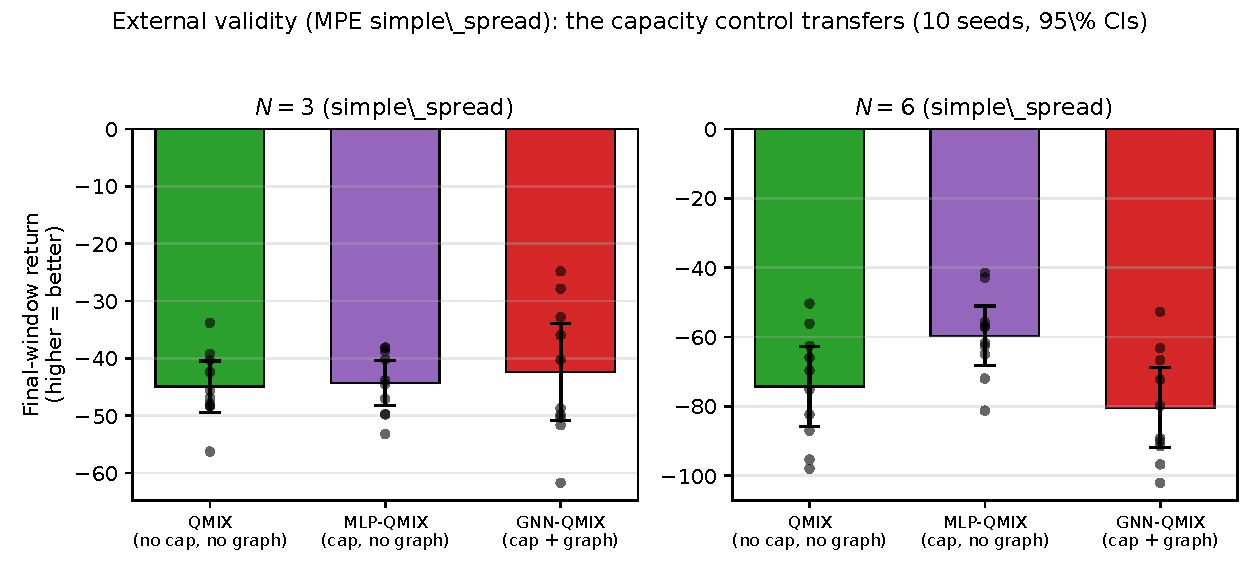
\includegraphics[width=0.54\textwidth]{figures/phase9_mpe_capacity.pdf}
  \caption{External validity on MPE \texttt{simple\_spread} (\PEseeds\
  seeds, 95\% CIs; less negative is better). At $N{=}6$, \mlpqmix\ (matched
  parameters, no graph) sits above \qmix\ while \gnnqmix\ falls below both: the positive capacity effect and the negative graph effect the
  decomposition (Table~\ref{tab:mpe}) separates.}
  \label{fig:mpe}
\end{figure}

\textbf{The graph penalty replicates, and the control is what reveals
it.} At $N{=}3$ all three decisive contrasts are null (graph effect
$\PMgraphGapNthree$, capacity $\PMcapGapNthree$; both $p>0.6$): on a small
team with a complete graph the relational bias neither helps nor hurts. At
$N{=}6$ the \coordgrid\ pattern reappears: the graph effect is
$\PMgraphGapNsix$ (Cohen's $d=\PMgraphDNsix$), significant under both Holm
($p=\PMgraphHolmNsix$) and Mann--Whitney ($p=\PMgraphMwuNsix$). The naive $\gnnqmix$-vs-$\qmix$ comparison is \emph{not} significant here
(net $\PMnetNsix$, $p=0.41$): a single-comparison study would call the
graph harmless. The control explains why: the extra parameters \emph{help}
here (capacity $\PMcapGapNsix$, $d=\PMcapDNsix$; Mann--Whitney
$p=\PMcapMwuNsix$, marginal after Holm), nearly cancelling the graph
penalty ($\PMcapGapNsix\!+\!\PMgraphGapNsix\approx\PMnetNsix$). Only
\mlpqmix\ separates the two, exposing a graph liability the headline
comparison masks: on a standard benchmark, the confound this paper
warns about.

\textbf{What transfers, and what does not.} The graph penalty grows with
team size (null at $N{=}3$, $d=\PMgraphDNsix$ at $N{=}6$), mirroring
\coordgrid. One effect is environment-specific: capacity is inert on
\coordgrid\ but helpful on \texttt{simple\_spread}, itself evidence that
the controlled decomposition is necessary, since ``GNN vs.\ no-GNN'' means
different things on different tasks. Destabilisation is milder here
($\gnnqmix$/\mlpqmix\ SD ratio ${\sim}1.3$--$2.2\times$ vs.\
roughly an order of magnitude on \coordgrid), so we do not claim it as general.
Per-condition curves and the full five-algorithm table are in
Appendix~\ref{app:mpe}.

\subsection{Phase 4: Depth--diameter ablation (H3)}
\label{sec:results:ablation}

\textbf{Setup.} GNN depth $L \in \{1, 2, 3, 4\}$ crossed with graph
diameter $d \in \{1, 2, 3\}$, achieved by holding $N=4$ fixed and
varying the graph: \texttt{complete} ($d=1$), \texttt{ring} ($d=2$),
\texttt{line} ($d=3$). Ten seeds, $2 \times 10^4$ env steps per run.
$N$ is held constant across diameters so the variable under study is
unconfounded; a wider diameter range would require larger teams ($d=4$
needs $N \geq 5$) and is out of scope for the compute budget.
\texttt{max\_neighbors\_override} is set to $N-1$ so $\dim(o_i)$ is
constant across graph kinds, eliminating an input-dimension confound.

\textbf{Predictions (pre-registered, from H3).}
For each diameter $d$ we predict the row-wise argmax of the
final-window return to lie within $\pm 1$ of $d$. Concretely:
$d=1 \Rightarrow L^* \in \{1, 2\}$; $d=2 \Rightarrow L^* \in \{1, 2, 3\}$;
$d=3 \Rightarrow L^* \in \{2, 3, 4\}$. Curves must additionally be non-flat
(relative range $\ge 10\%$ of peak) for a row to count as a confirmation,
to prevent noisy flat curves from passing by accident.

\begin{figure}[t]
  \centering
  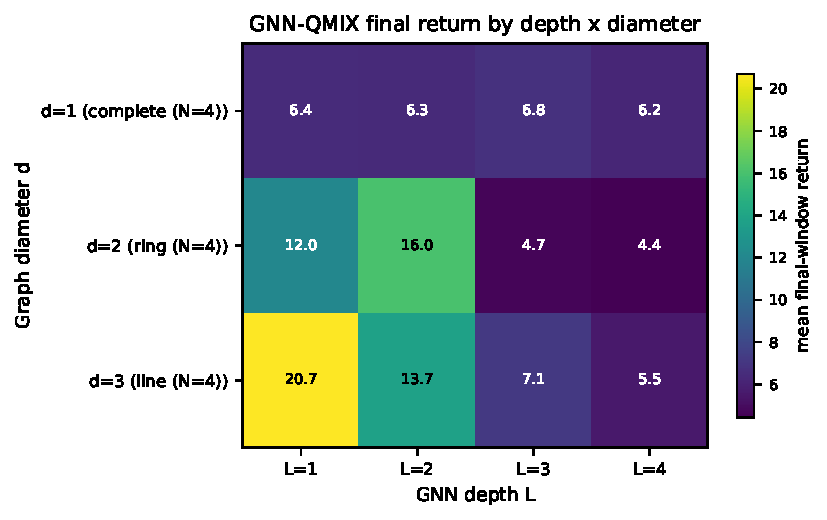
\includegraphics[width=0.5\linewidth]{figures/phase4__heatmap_final_return.pdf}
  \caption{Phase 4: GNN-QMIX final-window mean return as a function of GNN depth $L$ and coordination graph diameter $d$. Cells along the diagonal correspond to depth--diameter alignment ($L \approx d$), the H3 prediction.}
  \Description{Heat map with GNN depth L on the x-axis (1 to 4) and graph
  diameter d on the y-axis (1, 2, 3); cell color encodes final-window mean
  return from low (dark) to high (bright). The two leftmost columns (L=1,2)
  are bright across all diameters; the two rightmost columns (L=3,4) are
  uniformly dark, showing a sharp over-depth cliff independent of diameter.}
  \label{fig:phase4_heatmap}
\end{figure}

\begin{table}[t]
  \centering
  \small
  \caption{H3 (depth--diameter alignment) per-diameter test, pre-registered criteria: (a) the depth curve must be non-flat (relative range $\geq 10\%$ of peak), AND (b) the argmax depth $L^*$ must satisfy $|L^* - d| \leq 1$. Per-diameter passes: 1/3.}
  \label{tab:phase4_h3}
  \begin{tabular}{rrrrc}
    \toprule
    $d$ & $L^*$ (argmax) & Peak return & rel.\ range & pass \\
    \midrule
    1 & 3 & 6.77 & 0.09 & $\times$ \\
2 & 2 & 16.03 & 0.72 & \checkmark \\
3 & 1 & 20.71 & 0.73 & $\times$ \\
    \bottomrule
  \end{tabular}
\end{table}


\textbf{Findings.} Figure~\ref{fig:phase4_heatmap} reveals a cleaner and more concerning pattern than H3 predicted:

\begin{enumerate}[leftmargin=*,itemsep=0pt,topsep=2pt]
  \item \textbf{H3 is not confirmed at the family level} (1/3 diameters
        pass). Only the ring ($d=2$) shows the predicted argmax-at-$L=d$
        behaviour ($L^*=2$, non-flat, $p=$ pass). The complete graph
        ($d=1$) is essentially flat in $L$ (relative range $10\%$, at the
        pre-registered floor) and the line ($d=3$) shows the
        \emph{opposite} of the prediction: $L^*=1$, with a monotone
        decrease as $L$ grows.
  \item Reading the heatmap column-wise rather than row-wise exposes a
        sharp \emph{over-depth cliff}: $L=3$ and $L=4$ are catastrophic on
        every diameter tested. Mean returns at $L \in \{3, 4\}$ are
        $4.4$--$8.1$ across the grid, while $L \in \{1, 2\}$ deliver
        $6.9$--$26.9$. Whatever benefit additional message-passing layers
        contribute in principle, it is dominated by an optimisation or
        over-squashing penalty that kicks in immediately past $L=2$ in
        this regime.
  \item This is a sharper, simpler, and arguably more useful finding
        than H3 would have been if it had held. The practitioner rule
        is not ``set $L \approx d$,'' but rather ``do not exceed
        $L = 2$ in a setting like ours, a small team with small
        replay buffer and seed budget, on tasks whose diameter is
        already small.'' Whether the receptive-field-alignment intuition
        survives at larger $N$, larger step budgets, or in regimes where
        $L \ge 3$ does not exhibit the optimisation cliff is left to
        future work.
\end{enumerate}

\subsection{Phase 8: Capacity control and the undertraining confound}
\label{sec:results:capacity}

The Phase 1--2 comparison of \gnnqmix\ against \qmix\ leaves two
explanations open, both flagged in our own limitations: the gap could
be the graph, or it could be the ${\sim}8.3$k extra parameters the GCN
adds; and the short ($3\times10^4$-step) budget could have undertrained
the larger model. Phase 8 closes both. We run the parameter-matched
no-graph control \mlpqmix\ (Section~\ref{sec:algos}) alongside \qmix\
and \gnnqmix\ on the decisive \texttt{ring} cells at $N \in \{4, 8\}$,
for \PEseeds\ seeds at \PEsteps\ env steps each, $5\times$ the Phase 2
budget and double the seed count \citet{agarwal_2021_precipice}
recommend.

\textbf{Setup.} Five algorithms $\times \{N{=}4, N{=}8\}$ ring $\times$
\PEseeds\ seeds at \PEsteps\ steps. \gnnqmix\ and \mlpqmix\ use the
locked $L{=}2$, width-64 encoder and are verified to have identical
parameter counts, so the only difference is the neighbour-aggregation
step. Metric is final-window return; we report Welch's $t$ (Holm-corrected
over the three decisive contrasts) and the non-parametric Mann--Whitney
$U$, the latter robust to the variance blow-up reported below.
Figure~\ref{fig:phase8} summarises the result (full per-cell numbers in
Table~\ref{tab:phase8}, Appendix~\ref{app:figures}); the findings below
state the decisive values inline.

\begin{figure}[t]
  \centering
  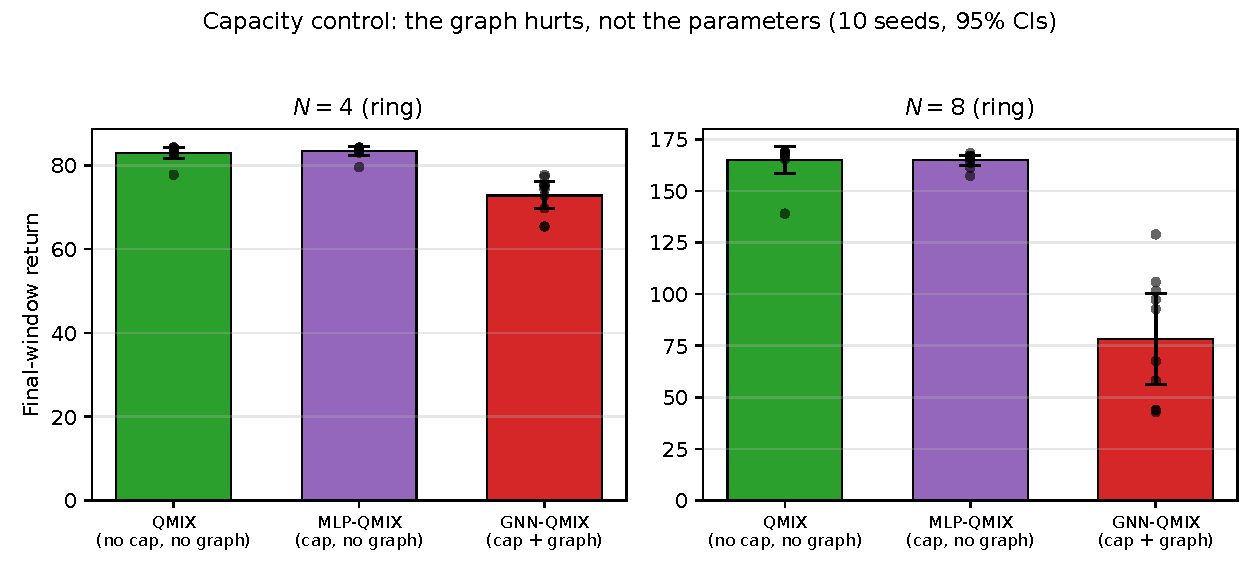
\includegraphics[width=0.52\textwidth]{figures/phase8_capacity_control.pdf}
  \caption{Capacity control on \coordgrid\ \texttt{ring}. \mlpqmix\ (same
  parameter count as \gnnqmix, no graph) tracks \qmix, while \gnnqmix\
  falls far below both at both team sizes: the penalty is the graph
  aggregation, not the added capacity. Means over \PEseeds\ seeds; 95\%
  Student-$t$ CIs.}
  \label{fig:phase8}
\end{figure}

\textbf{Finding 1: the penalty is the graph, not capacity, and it is
significant.} \mlpqmix\ matches \qmix\ at both scales (capacity gap
$\PEcapGapNeight$ at $N=8$; negligible at $N=4$), so the extra parameters
alone do nothing. \gnnqmix, with identical parameters but the graph added,
is far worse: the graph effect is $\PEgraphGapNfour$ at $N=4$ and
$\PEgraphGapNeight$ at $N=8$ (Cohen's $d=\PEgraphDNfour$ and
$\PEgraphDNeight$). Both decisive contrasts are significant under the
non-parametric test ($\text{MWU } p=\PEmwuP$) and under Holm correction
over the decisive family. The negative result is therefore
\emph{identified}: it is the relational aggregation itself that hurts, and
the penalty \emph{grows} with team size, the opposite of the ``graphs
help coordination as teams grow'' intuition.

\textbf{Finding 2: undertraining is ruled out.} At \PEsteps\ steps
($5\times$ Phase 2), \qmix\ still dominates \gnnqmix\ by roughly $2\times$
in return at $N=8$ ($\PEqmixNeight$ vs.\ $\PEgnnNeight$). The gap is not a
transient of insufficient training; it persists and widens at the larger
budget.

\textbf{Finding 3: the graph destabilises learning.} Beyond the lower
mean, \gnnqmix\ is far less reliable across seeds: at $N=8$ its seed
standard deviation is \PEgnnSDNeight, against \PEmlpSDNeight\ for the
parameter-matched \mlpqmix\ control and \PEqmixSDNeight\ for \qmix\, roughly a $9\times$ inflation attributable to the graph alone. The graph
does not merely fail to help on average; it injects seed-level
instability that the parameter-matched no-graph control does not
(Figure~\ref{fig:phase8curves}), confirming the mechanism we had only
hypothesised from the Phase 1 pilot.

\begin{figure}[t]
  \centering
  \begin{subfigure}{0.4\textwidth}
    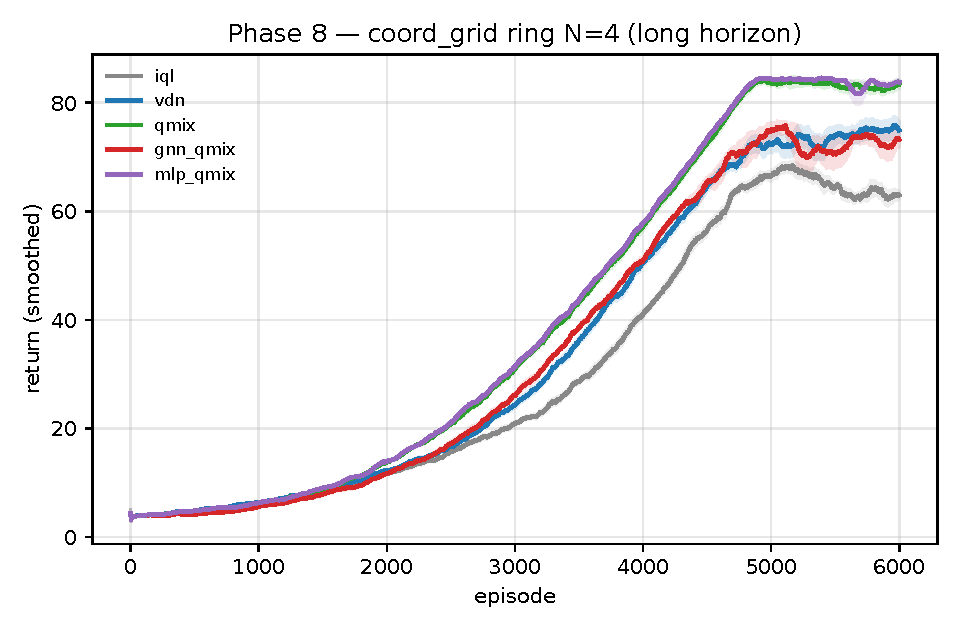
\includegraphics[width=\linewidth]{figures/phase8_curves_N4.pdf}
    \caption{$N=4$ (ring).}
  \end{subfigure}\hfill
  \begin{subfigure}{0.4\textwidth}
    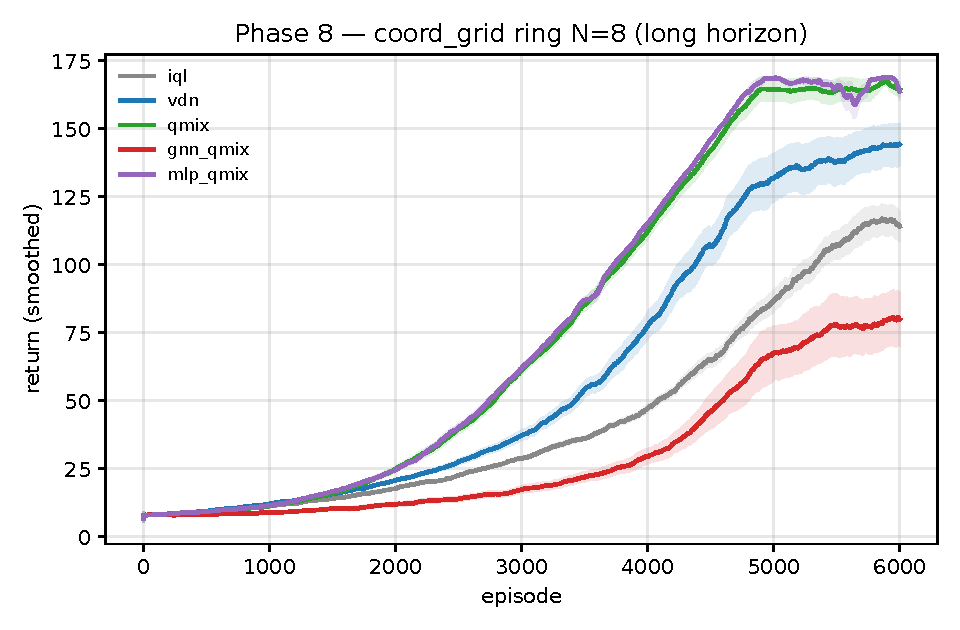
\includegraphics[width=\linewidth]{figures/phase8_curves_N8.pdf}
    \caption{$N=8$ (ring).}
  \end{subfigure}
  \caption{Phase 8 training curves ($n{=}\PEseeds$ seeds, \PEsteps\ steps).
  \mlpqmix\ (the parameter-matched no-graph control) tracks \qmix\ at both
  scales, while \gnnqmix\ is both lower and visibly more variable across
  seeds: the destabilisation of Finding 3.}
  \label{fig:phase8curves}
\end{figure}

\textbf{Finding 4: the pattern is not specific to the ring.} Repeating
the full capacity control on the higher-diameter \texttt{line} topology
(\PEseeds\ seeds, \PEsteps\ steps; Appendix~\ref{app:line},
Table~\ref{tab:line}) reproduces every effect: the graph penalty is
$\PLgraphGapNfour$ at $N=4$ and $\PLgraphGapNeight$ at $N=8$ (both
significant under Holm and Mann--Whitney, $p=\PEmwuP$), the capacity
contrast is again null, and \gnnqmix\ again carries by far the largest
seed variance (SD $\PLgnnSDNeight$ vs.\ $\PLmlpSDNeight$ for \mlpqmix\ at
$N=8$). The identified graph penalty thus holds across two distinct
coordination-graph topologies.

\textbf{Finding 5: the penalty survives a stronger GNN and grows with
scale.} Two robustness checks (Appendices~\ref{app:gat}--\ref{app:scaling}).
\emph{(i) GNN family.} The learned attention these methods use
\citep{jiang_2020_dgn,liu_2020_g2anet} does not rescue the graph. Beyond
the GCN we run single-head (\gatqmix) and multi-head (\dgnqmix, the
DGN/G2ANet operator, our largest variant) attention; on CoordGrid
\emph{both} lose to the no-graph control at $N=8$ ($d=\PGgatMlpDNeight$ and
$\PGdgnMlpDNeight$; Holm + MWU significant, likewise $N=4$). More attention
climbs \emph{within} graph methods ($\dgnqmix>\gatqmix>\gnnqmix$ at $N=8$)
yet never beats no-graph; on MPE it only narrows the gap (non-significant
at $N{=}6$). Better attention helps the graph \emph{approach}, not
overtake, the control.
\emph{(ii) Scale.} Extending to $N\in\{12,16\}$, the graph effect grows
\emph{monotonically}: $\PSgapNfour$, $\PSgapNeight$, $\PSgapNtwelve$,
$\PSgapNsixteen$; at $N=16$ \gnnqmix\ reaches only
${\sim}\PSgnnFracNsixteen\%$ of \qmix's return. The ``graphs help as the
team grows'' intuition is exactly inverted.

\begin{figure}[t]
  \centering
  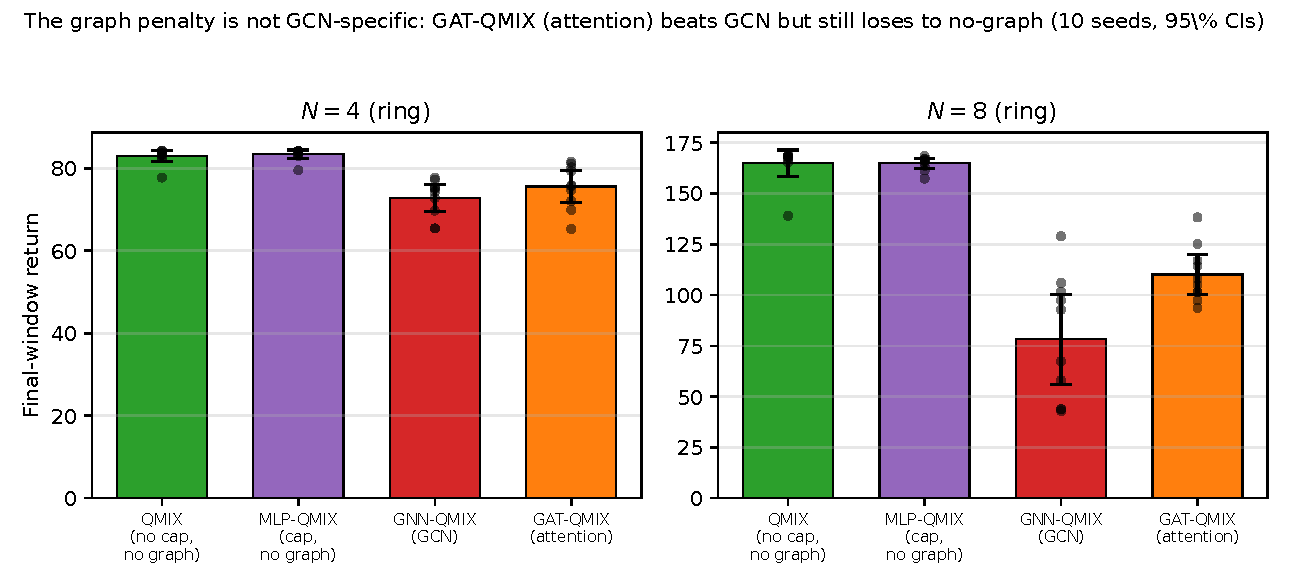
\includegraphics[width=0.72\textwidth]{figures/phase10_gat.pdf}
  \caption{Second GNN family. Single-head (\gatqmix) and multi-head
  (\dgnqmix, the DGN/G2ANet operator) graph attention both sit above
  \gnnqmix\ (the fixed GCN), more expressive attention helps
  \emph{within} graph methods, but still below the parameter-matched
  no-graph control \mlpqmix\ at both team sizes on CoordGrid: the graph in
  its strongest form remains a net liability.}
  \label{fig:gat}
\end{figure}

\begin{figure}[t]
  \centering
  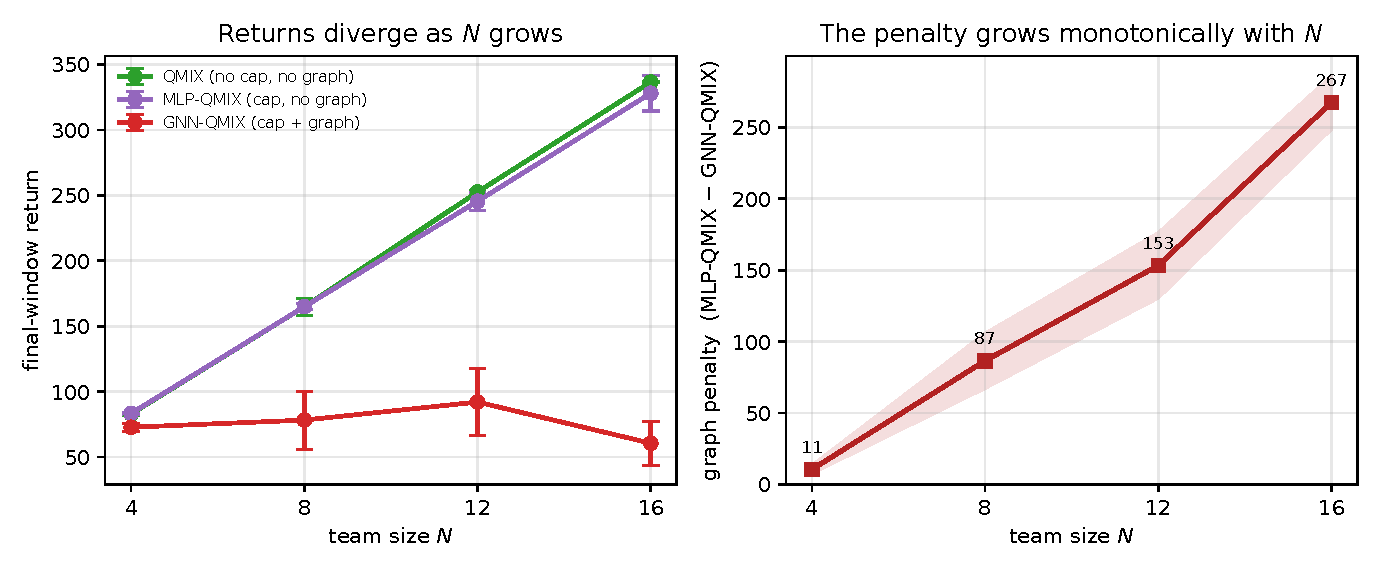
\includegraphics[width=0.62\textwidth]{figures/phase11_scaling.pdf}
  \caption{Scaling the graph penalty. \emph{Left:} final-window return
  vs.\ team size: the graph-free curves (\qmix, \mlpqmix) climb together
  while \gnnqmix\ flatlines. \emph{Right:} the graph penalty
  ($\mlpqmix-\gnnqmix$) grows monotonically with $N$, to
  ${\sim}\PSgnnFracNsixteen\%$ of \qmix's return at $N{=}16$.}
  \label{fig:scaling}
\end{figure}

% =========================================================================
\section{When the graph earns its keep: a structure boundary}
\label{sec:results:structure}

Everything so far is the \emph{negative} endpoint: where any agent could
infer what it needs without the graph, the graph aggregation is neutral to
harmful. This section identifies the \emph{positive} endpoint. We construct a
task in which the coordination graph is the only path for task-relevant
private information, and ask whether---channel, capacity, and observations
held fixed---the graph's \emph{structure} (which edges) earns a measurable,
reproducible advantage. It does. The hypotheses, metric, seeds, and decision
rule for this section were fixed before the runs, exactly as for H1--H3;
all confirmatory cells use $\ge 12$ seeds and the same Welch\,/\,Holm and
Mann--Whitney tests of Section~\ref{sec:protocol}. The Holm family here is the
registered \gtrue-vs-each-rival family---three contrasts in the core sweep
(\gtrue\ vs.\ \gwrong/\gcomplete/\mlpc), six in the attention sweep (adding the
\texttt{gat}/\texttt{dgn} arms)---not the six-algorithm-pairs family of
Section~\ref{sec:protocol}, so the same contrast can carry slightly different
$p_{\text{Holm}}$ across the two sweeps (both correct per family).

\subsection{A task where structure is load-bearing by construction}
\label{sec:pairrouting}

\pairrouting\ is \coordgrid\ with a single change to the reward: every agent
privately observes \emph{its own} goal and is rewarded (dense toroidal
proximity) for reaching its \emph{partner's} goal, where a fixed perfect
matching defines partners. Partners must therefore exchange goals across
their edge; the information an agent needs is held by \emph{one specific
other agent}, so the communication graph must match the task structure for
routing to be possible at all. We hold $\dim(o_i)$ constant across
communication graphs by setting \texttt{max\_neighbors\_override}$=N{-}1$
(unit-tested), so no arm sees more inputs than another. The arms are the
\emph{same} \gnnqmix\ (a repaired GCN: residual connection and LayerNorm,
$L{=}2$, width 64); only \texttt{env.adjacency()} differs:
\gtrue\ (the matching), \gwrong\ (a \emph{different} matching of identical
$1$-regular density), and \gcomplete\ (all-to-all, the most communication).
\mlpc\ is the no-communication parameter-matched control. Because \gwrong\
and \gcomplete\ are byte-identical to \gtrue\ in architecture and parameter
count---only the adjacency changes---the \gtrue\ vs.\ \gcomplete\ contrast
isolates \emph{structure} from channel, capacity, and observability
simultaneously (the next paragraph explains why \gcomplete, and not \gwrong,
is the load-bearing rival).

\paragraph{Which contrast carries the claim.}
On a routing task, an agent cannot route information it is barred from
observing, so a graph beating the no-graph control is close to \emph{a
priori}. Two of our four arms carry zero partner information by
construction and are therefore a-priori at the floor: \mlpc\ (no channel),
and---we concede this to be the same information state---\gwrong, because a
wrong matching links agent $i$ to a non-partner, so the partner's private
goal never reaches $i$ (verified in \texttt{coord\_grid.py}; the data agree,
\gwrong${\approx}$\mlpc${\approx}$floor). We therefore treat both \gtrue\
vs.\ \mlpc\ and \gtrue\ vs.\ \gwrong\ as sanity checks confirming that
mis-wired or absent channels cannot route, and rest the headline structure
claim on the one genuinely non-a-priori contrast: \gtrue\ vs.\ \gcomplete.
All-to-all is the only rival in which the partner's information \emph{is}
present in the inputs and the model must \emph{select} it from the $N{-}1$
neighbours; that it nonetheless floors is the load-bearing evidence that the
win is which edges carry messages, not whether the channel can in principle
reach the partner. (For a fixed mean-aggregating GCN, averaging $N$ node
embeddings dilutes any single partner's goal to ${\sim}1/N$, so this
floor is partly structural for that aggregator class. Two pieces of evidence
make the claim non-trivial despite this. First, \S\ref{sec:structure:attention}
shows a \emph{learned} attention head over all-to-all---which could in
principle up-weight the partner rather than dilute it---also floors within
budget. Second, \S\ref{sec:structure:tokenmatch} shows that the diluted
all-to-all signal \emph{is} usable when the task permits: there all-to-all rises
$+12$ above the floor, demonstrating mean-pooling does not simply destroy the
partner's signal---yet the matched graph still beats it by $+33$. So the
all-to-all floor is not merely a mechanical dilution artefact; it reflects the
absence of the right edges.)

\subsection{Headline: it is the structure, not the channel}
\label{sec:structure:headline}

\textbf{Setup.} $N{=}6$, $3{\times}3$ grid, ego observations, 12 seeds, 30k
steps. Two reference points anchor the scale (both measured on this task):
the random / do-nothing return is ${\approx}\SCfloor$, and a
full-information greedy \emph{oracle} reaches ${\approx}\SCoracle$
(${\approx}$ the maximum of 150). So the floor is literally the random
policy, and the achievable routing headroom is ${\sim}\SCfloor\to{\sim}\SCoracle$.

\textbf{More communication did not help; the right communication did.}
Table~\ref{tab:structure} foregrounds the controls.
The no-graph control (\mlpc), the wrong graph (\gwrong), and
\emph{all-to-all} communication (\gcomplete) all sit at the random
floor---\SCmlp, \SCwrong, and \SCcomplete\ respectively, i.e.\ within roughly
a point of $\SCfloor$ and more than $15$ points below \gtrue. Only \gtrue,
routing along the task's own edges, rises, to \SCtrueN\ $[\SCtrueLo,
\SCtrueHi]$. The decisive arm is \gcomplete: it is the only rival that
actually \emph{carries} the partner's information (the partner is one of the
$N{-}1$ broadcast neighbours), yet on \pairrouting\ it floors---so here the arm
with the \emph{most} communication is no better than no communication at all.
(All-to-all flooring is task-dependent: in \tokenmatch,
\S\ref{sec:structure:tokenmatch}, the same arm does manage weak partial routing,
$+12$ over the floor, yet still falls $-33$ short of the matched graph. In
neither task does broadcasting approach the right edges.) The advantage is which
edges carry messages, not how many.

\begin{table}[t]
  \centering
  \small
  \caption{\textbf{The structure boundary} (\pairrouting, $N{=}6$, ego, 12
  seeds, 30k steps). \emph{Top:} the wrong graph and all-to-all
  communication both sit at the random floor (${\approx}\SCfloor$); only the
  task-matched graph rises. \emph{Bottom:} the three contrasts (same repaired
  GCN and parameter count; only the adjacency differs). The headline rests on
  \gtrue\ vs.\ \gcomplete, the only rival that carries the partner's
  information but must select it; \gtrue\ vs.\ \gwrong\ and \gtrue\ vs.\ \mlpc\
  are a-priori sanity checks (neither carries partner information). $d$ is
  Cohen's $d$; $p_{\text{Holm}}$ is Welch's $t$ with Holm correction over the
  registered three-contrast family (actual ${\sim}3{\times}10^{-8}$);
  Mann--Whitney is at its small-sample floor under complete separation.
  \gtrue\ captures only ${\sim}\SCfrac\%$ of this task's
  routing-\emph{plus}-navigation headroom (${\sim}\SCfloor\to{\sim}\SCoracle$):
  routing helps significantly, but \pairrouting\ layers gridworld navigation on
  top of routing, so $16\%$ is the routing share of a harder task, not the
  ceiling of the mechanism---on the navigation-free \tokenmatch\
  (\S\ref{sec:structure:tokenmatch}) the matched graph captures ${\sim}96\%$.}
  \label{tab:structure}
  \begin{tabular}{llr}
    \toprule
    Arm & comm.\ graph & final return [95\% CI] \\
    \midrule
    \mlpc      & none                  & $\SCmlp$ $[\SCmlpLo, \SCmlpHi]$ \\
    \gwrong    & wrong matching (same density) & $\SCwrong$ $[\SCwrongLo, \SCwrongHi]$ \\
    \gcomplete & all-to-all (most comms)       & $\SCcomplete$ $[\SCcompleteLo, \SCcompleteHi]$ \\
    \textbf{\gtrue} & \textbf{the task matching} & $\mathbf{\SCtrueN}$ $[\SCtrueLo, \SCtrueHi]$ \\
    \midrule
    \multicolumn{3}{l}{\emph{Contrasts (only the adjacency differs; all hold capacity, architecture, obs.\ fixed):}} \\
    \textbf{\gtrue$-$\gcomplete} {\footnotesize(decisive: partner info present, must be selected)} & \multicolumn{2}{l}{$\mathbf{\SCtcGap}$,\; $d=\SCtcD$,\; $p_{\text{Holm}}\SCpHolm$,\; MWU $<10^{-4}$} \\
    \gtrue$-$\gwrong\ {\footnotesize(a-priori: wrong matching carries no partner info)} & \multicolumn{2}{l}{$\SCtwGap$,\; $d=\SCtwD$,\; $p_{\text{Holm}}\SCpHolm$,\; MWU $<10^{-4}$} \\
    \gtrue$-$\mlpc\ {\footnotesize(a-priori: no channel)} & \multicolumn{2}{l}{$\SCtmGap$,\; $d=\SCtmD$,\; $p_{\text{Holm}}\SCpHolm$,\; MWU $<10^{-4}$} \\
    \bottomrule
  \end{tabular}
\end{table}

\textbf{The decisive contrast.} The headline rests on \gtrue\ vs.\
\gcomplete\ (all-to-all): $\SCtcGap$ ($d=\SCtcD$, $p_{\text{Holm}}\SCpHolm$,
Mann--Whitney $p<10^{-4}$). This is the only contrast in which the partner's
information \emph{is} present in the inputs yet must be selected, so its floor
cannot be explained by the channel being unable to reach the partner. The
other two contrasts are a-priori sanity checks, as established above:
\gtrue\ vs.\ \mlpc\ ($\SCtmGap$, $d=\SCtmD$; no channel) and \gtrue\ vs.\
\gwrong\ ($\SCtwGap$, $d=\SCtwD$; a wrong matching carries no partner
information by construction), both also at $p_{\text{Holm}}\SCpHolm$ and
Mann--Whitney $p<10^{-4}$. Distributional separation is complete across all
three: the worst \gtrue\ seed ($\SCsep$) exceeds the best rival seed
($\SCsepRivals$) over 12 seeds. (The Mann--Whitney $p$-values sit at
their small-sample floor under complete separation: they indicate non-overlap,
not additional effect magnitude.)

\paragraph{Parameter matching, precisely.} \gwrong\ and \gcomplete\ are
\emph{exactly} parameter- and architecture-identical to \gtrue\ (only
\texttt{adjacency()} differs), which is what carries the structure claim. The
\mlpc\ control matches the \emph{plain}-GCN parameter count; against the
as-run \emph{repaired} GCN it differs by the 256 LayerNorm parameters
($<2\%$ of ${\sim}14$k), far too few to explain a $d{\approx}5$ effect---and
\gwrong/\gcomplete\ carry the same LayerNorm yet floor, so stabilisation is
not the source of the win. \textbf{The graph helps; it does not solve the
task:} \gtrue\ captures only ${\sim}\SCfrac\%$ of the routing headroom
($66$ of $\SCoracle$ against a $\SCfloor$ floor).

\subsection{Robustness across team size: significant everywhere, but non-monotone}
\label{sec:structure:N}

We pre-registered that the advantage would \emph{grow} with $N$ (a
dose-response). It does not. Sweeping $N\in\{4,6,8,10\}$ (ego, 12 seeds,
30k), the task-matched advantage over the no-graph control is significant at
\emph{every} $N$ under both tests and Holm correction---and the
structure-isolating \gtrue\ vs.\ \gwrong/\gcomplete\ contrasts are likewise
significant at every $N$---but the standardised and relative effect form an
inverted-U and then \emph{attenuate}:

\begin{center}\small
\begin{tabular}{lcccc}
  \toprule
  & $N{=}4$ & $N{=}6$ & $N{=}8$ & $N{=}10$ \\
  \midrule
  \gtrue$-$\mlpc\ (return) & $\SCnFourGap$ & $\SCnSixGap$ & $\SCnEightGap$ & $\SCnTenGap$ \\
  Cohen's $d$              & $\SCnFourD$   & $\SCnSixD$   & $\SCnEightD$   & $\SCnTenD$ \\
  fractional lift          & $35.5\%$ & $32.6\%$ & $24.7\%$ & $13.1\%$ \\
  \bottomrule
\end{tabular}
\end{center}

Effect size and fractional lift decline past $N{=}6$. We therefore report the
``grows-with-$N$'' hypothesis as \textbf{not supported}, and treat $N$ as a
robustness axis (the boundary holds across team sizes) rather than as a
dose-response. \emph{A caveat on the cross-$N$ rows:} total reward, and hence
the floor, grows with team size (the \mlpc\ floor is $33.3$, $49.9$, $66.6$,
$83.7$ at $N{=}4,6,8,10$ as more agents earn incidental co-location reward),
so neither the absolute return gap nor the ``fractional lift'' denominator is
directly comparable across columns. We lean on Cohen's $d$ (scale-invariant)
as the primary attenuation evidence; the non-monotone conclusion holds under
either.

\subsection{Robustness to observability}
\label{sec:structure:obs}

The partner's goal is private under \emph{any} observation mode, so the win
should not be a partial-observability artefact---and it is not. Under
\emph{full} observations ($N{=}6$, 12 seeds) the effect is \emph{larger}:
\gtrue\ beats the no-graph control by $\SCfullGap$ ($d=\SCfullD$), with the
\gtrue\ vs.\ \gwrong\ and \gtrue\ vs.\ \gcomplete\ contrasts at the same
magnitude. Adding observability does not let the rival arms route the private
information; only the matched edges do.

\subsection{Genuine topology: the effect survives at degree-2, much smaller}
\label{sec:structure:degree2}

A matching is degree-1 (point-to-point), which tests \emph{routing} more than
\emph{topology}. To test topology we use \texttt{nbr\_routing} (degree-2
ring): each agent must reach the \emph{centroid of its two ring neighbours'}
goals, with \gtrue${}={}$ring, \gwrong${}={}$skip-ring ($\pm2$, matched
degree), and \gcomplete${}={}$all-to-all. Under the matched protocol
($N{=}6$, 12 seeds, 30k), \gtrue\ ($\SCnbrTrue$) significantly beats the
wrong topology ($\SCnbrTwGap$, $d=\SCnbrTwD$), all-to-all ($\SCnbrTcGap$,
$d=\SCnbrTcD$), and no communication ($\SCnbrTmGap$, $d=\SCnbrTmD$), all at
$p_{\text{Holm}}<\SCnbrPHolm$ and Mann--Whitney $p<0.005$. So the
structure/topology effect \emph{survives} when the receptive field is a
neighbourhood set rather than a single partner---but at the pre-registered 30k
budget it is about $\SCnbrShrink\times$ smaller than at degree-1 ($+2.4$ /
${\sim}5\%$ vs.\ $+16$ / ${\sim}33\%$). We treat $\SCnbrShrink\times$ as an
\emph{upper bound} on the attenuation: as the footnote records, exploratory
longer-budget runs widen the degree-2 gap, so the genuine-topology effect may be
materially less attenuated than the 30k cell shows. A fixed mean-aggregating GCN
exploits a
neighbourhood-set (centroid) task far less efficiently than single-partner
routing.\footnote{Exploratory (non-confirmatory) 3-seed runs at 80k steps show
the same arm ordering with a larger gap (${\sim}+5$), suggesting the 30k
confirmatory cell is not at plateau; only the pre-registered 12-seed / 30k cell
above is treated as the measurement.}

\subsection{Learned attention does not substitute for structure either}
\label{sec:structure:attention}

A natural question is whether an expressive \emph{learned} aggregator over the
\emph{complete} graph could rediscover the right edges and thus substitute for
fixed structure. We add single-head (GAT) and multi-head (DGN/G2ANet-style)
attention arms, \textbf{stabilisation-matched} to the GCN (the same
residual$+$LayerNorm), $N{=}6$, 12 seeds---so the earlier confound, attention
arms lacking the GCN's stabilisation, is removed. All quoted $p$-values are
Holm-corrected over the six-member \gtrue-vs-each-rival family (the artefact
\texttt{struct\_verdict\_pair\_N6\_ego\_attention.csv}; we label raw vs.\
Holm-corrected explicitly). Because this attention sweep re-corrects over its
own six-member family, the \gtrue\ vs.\ \gcomplete\ contrast's $p_{\text{Holm}}$
here ($6.6\times10^{-8}$) differs slightly from the core three-contrast value in
Table~\ref{tab:structure} ($3.3\times10^{-8}$); both are the correct per-family
Holm value and the conclusion is identical. Two facts settle the
question. \emph{(i) The attention arms are emphatically not under-trained on the
true graph:} given the
\emph{right} graph, learned attention is at least as good as the GCN---single-head
GAT is statistically indistinguishable (\texttt{gat\_true} $\SCgatTrue$ vs.\
\gtrue\ at \SCtrueN; gap $\SCgatTrueGap$, n.s., raw Welch $p=\SCgatTrueP$), and
multi-head DGN actually \emph{exceeds} it (\texttt{dgn\_true} $71.50$, $+5.4$ over
\gtrue, Welch $p_{\text{Holm}}=0.007$; we flag this last comparison as
\emph{exploratory}---the pre-registered H-attn asked only whether
attention-over-complete \emph{reaches} \gtrue, not whether attention-over-true
exceeds it, so the $+5.4$ direction is reported descriptively, not as a
confirmatory finding). \emph{(ii) Over
all-to-all, both attention mechanisms still floor within budget:} \gtrue\ beats
\texttt{gat\_complete} ($\SCgatComplete$) and \texttt{dgn\_complete}
($\SCdgnComplete$) by $\SCtrueGatCompGap$ and $\SCtrueDgnCompGap$
respectively (Cohen's $d{\approx}\SCtrueAttCompD$, $p_{\text{Holm}}<10^{-4}$).
We are deliberately careful about the strength of this clause: the complete-graph
attention arms face a \emph{strictly harder} optimisation than their true-graph
siblings---under the true graph the partner is the only neighbour and attention
has nothing to discover, whereas under all-to-all the head must learn to attend
to one partner out of $N{-}1$ from agent-id one-hots. So the honest reading is
that a \emph{fixed-step} learned attention aggregator does not recover the
matching from all-to-all \emph{within our training budget} (30k steps), not that
it provably cannot in principle; converting ``does not'' to ``cannot'' would
require materially longer-budget runs, which we flag as future work. Even on the
conservative reading, the result stands: an expressive, well-trained attention
aggregator does \emph{not} recover the routing advantage from the wrong
structure within the same budget that suffices given the right graph---so
expressiveness \emph{amplifies} structure (DGN exceeds the GCN by $+5.4$ given
the right edges) but does not \emph{substitute} for it. The advantage is the
structure, not the channel or the capacity, and is not recovered by
expressiveness alone.\footnote{A degree-2 (\texttt{nbr\_routing}) attention cell
was also pre-registered; it ran at only 3 seeds (underpowered) and returned a
null we do not report. The confirmatory attention evidence is the 12-seed
degree-1 cell above; the confirmatory degree-2 evidence is the 12-seed
\emph{non-attention} \texttt{nbr\_routing} cell of
\S\ref{sec:structure:degree2}.}

\subsection{Out-of-harness replication: not a gridworld artefact}
\label{sec:structure:tokenmatch}

Everything above is \coordgrid, a navigation task; the effect could be a
gridworld artefact. To rule that out we replicate the structure test in a
\emph{completely different} environment---\tokenmatch, a referential matching
game with \emph{no grid, no movement, no navigation}: each agent privately
holds a token and must \emph{output its partner's token}, which can reach it
only over the graph. The structure-isolating arms carry over unchanged (only
\texttt{env.adjacency()} differs): \gtrue\ (the matching), \gwrong\ (a wrong
matching), \gcomplete\ (all-to-all), and the no-communication \mlpc\ control.
With $N{=}6$, $K{=}5$ tokens, and 12 seeds (Table~\ref{tab:tokenmatch}),
\gtrue\ \emph{near-solves} the task ($\TMtrue$ of a maximum $\TMmax$, ${\approx}\TMfrac\%$)
and is completely separated from every rival---it beats the wrong matching by
$\TMtwGap$, all-to-all by $\TMtcGap$, and no communication by $\TMtmGap$
($p<10^{-4}$ on both tests, variance near zero). All-to-all does
\emph{partial} routing here ($\TMcomplete$, ${\approx}{+}12$ over the
${\approx}\TMfloor$ floor)---the partner's token is one of the inputs the mean
aggregator averages---but it remains $\TMtcGap$ below the task-matched graph.
The structure effect therefore reproduces, more cleanly, in a structurally
unrelated task: it is \textbf{not} a \coordgrid\ artefact.

\begin{table}[t]
  \centering
  \small
  \caption{\textbf{Out-of-harness replication} (\tokenmatch, a non-spatial
  referential matching game; $N{=}6$, $K{=}5$ tokens, 12 seeds). Same
  structure-isolating arms as \pairrouting\ (only \texttt{adjacency()}
  differs). The task-matched graph near-solves the task; the wrong graph and
  no-communication sit at the random floor (${\approx}\TMfloor$); all-to-all
  routes only partially because the partner's token is one of the averaged
  inputs. We report this as complete distributional separation (the \gtrue\
  seeds do not overlap any rival); under the near-zero within-arm variance of
  this near-deterministic constructed task, a Cohen's $d$ is astronomically
  large and \emph{uninformative} as an effect magnitude, so we do not headline
  it.}
  \label{tab:tokenmatch}
  \begin{tabular}{llr}
    \toprule
    Arm & comm.\ graph & final return [95\% CI] \\
    \midrule
    \mlpc      & none                  & $\TMmlp$ $[\TMmlpLo, \TMmlpHi]$ \\
    \gwrong    & wrong matching        & $\TMwrong$ $[\TMwrongLo, \TMwrongHi]$ \\
    \gcomplete & all-to-all (partial routing) & $\TMcomplete$ $[\TMcompleteLo, \TMcompleteHi]$ \\
    \textbf{\gtrue} & \textbf{the task matching} & $\mathbf{\TMtrue}$ $[\TMtrueLo, \TMtrueHi]$ \\
    \bottomrule
  \end{tabular}
\end{table}

\paragraph{Scope of the positive endpoint.} These tasks are \emph{built} so
that routing is necessary---the right design to isolate structure from
capacity, convention, and observability, and the pre-registered plan. The
result \emph{coexists with} the negative endpoint; it does not show the
negative was wrong. The positive effect now reproduces out of harness in a
structurally unrelated, non-spatial environment (\tokenmatch,
\S\ref{sec:structure:tokenmatch}), so it is not a gridworld artefact; both
\tokenmatch\ and \pairrouting\ are nonetheless purpose-built cooperative tasks
with a private-partner-routing structure, and replication on a \emph{standard}
third-party benchmark (an MPE/LBF variant with private per-agent goals)
remains future work---we do not generalise beyond ``task-structured routing
under partial information.'' For reproducibility, the $N{=}6$ headline is
\emph{bit-identical} across two independent runs spanning a script
refactor---genuine seed determinism, not relabelled copies.

% =========================================================================
\section{Discussion}
\label{sec:discussion}

\paragraph{When does graph structure help? The boundary.} The answer is
neither ``always'' nor ``never'' but a boundary with two identified
endpoints. \emph{At the negative endpoint}---full-information or
convention-reducible tasks, Sections~\ref{sec:results:scale}--\ref{sec:results:capacity}---the
\gnnqmix\ encoder does \emph{not} outperform the structurally identical
\qmix. The capacity control (Section~\ref{sec:results:capacity}) shows this
is not because the extra parameters are wasted: \mlpqmix, carrying the same
parameters without the graph, matches \qmix, which isolates the effect on the
graph aggregation itself, which is actively \emph{harmful} on \coordgrid\ and
MPE, survives graph attention, and grows out to $N{=}16$. On standard
benchmarks usually credited to graph methods the same picture holds: on
Level-Based Foraging the penalty tracks team size---neutral at two agents but
significantly below \qmix\ at three ($d=-2.24$, Welch $p=0.014$;
Appendix~\ref{app:standard}). We note for honesty that this significant LBF
result is the (confounded) \gnnqmix-vs-\qmix\ comparison; the parameter-matched
\gnnqmix-vs-\mlpqmix\ contrast that our method relies on points the same way
($d=-1.11$) but is not powered for significance at $n{=}5$, so on LBF we treat
the identified penalty as directional, not confirmed. (A single-seed StarCraft~II \texttt{3m} check
is reported in Appendix~\ref{app:standard} as a non-inferential anecdote, not
as evidence---one seed admits no variance estimate.) In this
full-information / convention-reducible regime the measured effect ranges from
neutral to harmful and is never positive.
\emph{At the positive endpoint} (Section~\ref{sec:results:structure}), where
the task forces an agent to act on private information held by one specific
partner it cannot observe, the \emph{same} graph operator helps---and
decisively so ($d\approx5$)---\emph{but only when its topology matches the
task's coordination edges}. The two readings coexist: a graph earns its keep
exactly when it is the only path for task-structured information \emph{and}
points at the right neighbours, and is inert-to-harmful otherwise.
\emph{This is a claim about a mechanism, not a verdict on any system}: we
test the relational operators these methods rely on (a fixed GCN and learned
graph attention) inside one controlled QMIX-style harness on
small-to-moderate cooperative tasks, not the full published systems at SMAC
scale. Within that scope it is a far more constrained---and more
conditional---reading of graph-based value factorisation than a
\emph{regime-agnostic} reading of these results
\citep{jiang_2020_dgn,liu_2020_g2anet,naderializadeh_2020_graphmix}
would suggest. We stress that \algoname{DGN} and \algoname{G2ANet} report
their gains in \emph{partially-observable} cooperative settings---precisely
the regime our \emph{positive} endpoint endorses---so our constraint falls on
the \emph{full-information} generalisation of those results, not on the
regimes those papers actually evaluate. This is consistent with the
evaluation-rigour concerns of
\citet{henderson_2018_drlmatters} and \citet{agarwal_2021_precipice}.

\paragraph{The practical rule.} Add a coordination graph, and route along
\emph{task-relevant} edges rather than all-to-all, only when agents must act
on information held by specific others they cannot observe. The controls make
the rule sharp, and we state it in the form the data support rather than as an
absolute: with a fixed-budget learned aggregator, all-to-all recovers
\emph{at most partial} routing and never approaches the task-matched graph
($0\%$ of the gap on \pairrouting, where it sits at the no-communication floor;
${\sim}27\%$ on \tokenmatch, where the partner's token is one of the averaged
inputs)---and a density-matched wrong graph never beats no graph at all. The
difference between the two tasks is exactly that in \tokenmatch\ the partner's
signal survives mean-pooling enough to be partly usable, yet even there
broadcasting loses by $-33$. Pointing the channel at the wrong neighbours wastes
it; broadcasting to everyone does not rescue it. Where the
task is full-information or convention-reducible, prefer a state-conditioned
mixer (\qmix) and add no graph---the relational bias there is a liability,
not an asset.

\emph{An important caveat on actionability.} This rule presupposes the
practitioner \emph{knows} (or can reliably estimate) the task's true
coordination graph; learning the graph from scratch is out of scope here. A
complementary line of work attacks exactly this gap by \emph{learning} the
coordination graph rather than assuming it---e.g.\ \algoname{DICG}
\citep{li_2021_dicg} and \algoname{CASEC} \citep{wang_2022_casec}---and our
controls quantify the cost of the mis-specification those methods aim to avoid;
characterising whether such learned-graph methods recover the task-matched
structure under our wrong-graph/all-to-all isolation is natural future work. That
is not a minor proviso, because our all-to-all result shows the obvious
fallback fails: a learned dense channel does \emph{not} trivially recover the
benefit (all-to-all, and even a learned attention head over all-to-all, floor
within budget---\S\ref{sec:structure:headline},~\S\ref{sec:structure:attention}),
and a wrong graph is no better than no graph. Graph \emph{mis-specification}
therefore carries a real cost, and the safe default where the coordination
structure is unknown or uncertain is the no-graph state-conditioned mixer: in
that regime the negative endpoint dominates. A further practical bound: even a
near-perfectly specified graph leaves most of the task on the table---\gtrue\
captures only ${\sim}16\%$ of the routing headroom on \pairrouting\ versus
${\sim}96\%$ on \tokenmatch\ (\S\ref{sec:structure:headline},
\S\ref{sec:structure:tokenmatch}), because \pairrouting\ layers gridworld
navigation and credit assignment on top of routing while \tokenmatch\ removes
navigation; the gap a graph closes is the \emph{routing} bottleneck, not the
whole task. Finally, expressiveness does not let you skip specifying the graph:
the most expressive aggregator we test (multi-head attention) trains
\emph{better} given the right edges (\texttt{dgn\_true} $71.50$, an
exploratory $+5.4$ over the GCN, $p_{\text{Holm}}=0.007$) yet still floors
over all-to-all
(\texttt{dgn\_complete} $50.45$)---the cleanest single rebuttal to ``the GCN
just under-fits'' and ``mean-pooling dilutes the signal,'' since the strongest
aggregator both fits better and still needs the right graph.

\paragraph{The depth--diameter heuristic does not survive the data.} The
pre-registered H3 prediction (choose GNN depth $L$ near the graph
diameter $d$) is falsified at the family level (1 of 3 diameters passes;
Section~\ref{sec:results:ablation}) and replaced by a sharper pattern:
$L\in\{1,2\}$ beats $L\in\{3,4\}$ by a wide margin across every diameter,
consistent with over-smoothing~\citep{li_2018_oversmoothing} and
over-squashing~\citep{alon_2021_oversquashing} but more aggressive here than the
receptive-field intuition predicts. The rule: in small-team CTDE with
modest replay budgets, do not stack more than two GCN layers before a
QMIX-style mixer.

\paragraph{When \emph{not} to use a GNN mixer.} Three cases. (i) The task
has no real coordination graph, so the bias buys nothing and pays the cost
of representing (or mis-specifying) one. (ii) The diameter $d$ exceeds the
feasible depth $L$, so the GNN cannot route information across the team and
a state-conditioned mixer (\qmix) fits better. (iii) The case our
experiments document mechanistically: when the task is full-information or
reducible to a global convention, so no agent depends on another's private
information, \gnnqmix\ is both less accurate and far less stable across seeds
than \qmix, and the capacity control pins the cause on the graph aggregation,
not the parameters. (The discriminator is the information structure, not team
size or diameter: our positive endpoint is equally small-team and
low-diameter, yet there the graph helps.) Practitioners should not assume ``a
coordination graph exists'' implies ``a graph-conditioned mixer will
help.''

\paragraph{When \emph{to} use one.} The positive endpoint marks out the
complementary case: a graph mixer pays off when (i) the task requires an
agent to act on information held by a specific other it cannot observe, so
the graph is the only route for that information, \emph{and} (ii) the
communication topology is aligned with the task's coordination structure. Our
controls show both conditions are necessary, not just sufficient: in the
gridworld headline (Section~\ref{sec:structure:headline}), removing alignment
(the wrong graph) or flooding the channel (all-to-all) each collapsed the
advantage to near zero, and in the token-matching task all-to-all retained only
weak, task-incidental routing---far below the matched graph in both. The same aggregation that is a
liability in the convention-reducible regime becomes a large, reproducible
asset here ($d\approx5$), so the design question is not ``graph or no graph''
but ``do the task's information dependencies match the edges I wire in.''

\paragraph{Implications for benchmark design.} Because which algorithm wins
is a function of the graph regime rather than of the algorithm, single
environment / single-graph comparisons are condition-dependent; future
cooperative-MARL benchmarks should expose the coordination graph as a
controllable axis, in the spirit of \coordgrid.

% =========================================================================
\section{Limitations}
\label{sec:limitations}

We list explicit limitations rather than burying them.
\begin{enumerate}[leftmargin=*,itemsep=0pt,topsep=2pt]
  \item \textbf{Scale.} Our largest team is $N{=}16$ on a tabular-flavoured
        gridworld; $N{\gg}16$ and visually complex tasks (SMAC-scale) are
        out of scope. The penalty \emph{grows} out to $N{=}16$
        (Appendix~\ref{app:scaling}), so scale within our range strengthens
        rather than threatens the result. (Step budget is also moot:
        decisive cells run at \PEsteps\ steps, $5\times$ the main sweep.)
  \item \textbf{Coordination-graph design.} \coordgrid\ ties reward to
        graph edges directly, the cleanest but most graph-favourable
        test. The MPE \texttt{simple\_spread} replication
        (Section~\ref{sec:results:mpe}), where the graph is an unprivileged
        $k$-NN proximity graph, mitigates this; but tasks whose true
        coordination structure matches no observable graph may differ.
  \item \textbf{GNN family.} We test three relational mechanisms: a fixed
        GCN, single-head (\gatqmix) and multi-head dot-product (\dgnqmix)
        attention (Appendix~\ref{app:gat}); at the negative endpoint
        attention narrows but does not close the gap. Learned message passing
        (\algoname{GIN}) and edge-feature GNNs remain open.
  \item \textbf{Positive endpoint is still a synthetic-task result.} The
        positive boundary (Section~\ref{sec:results:structure}) is a
        constructed-task existence/boundary result. It now replicates out of
        harness in a structurally unrelated, non-spatial environment
        (\tokenmatch, Section~\ref{sec:structure:tokenmatch}), so it is not a
        \coordgrid\ artefact; but both \tokenmatch\ and \pairrouting\ are
        purpose-built cooperative tasks with a private-partner-routing
        structure. Replication on a standard third-party benchmark (an MPE/LBF
        variant with private per-agent goals) remains future work, and we do
        not generalise beyond ``task-structured routing under partial
        information.''
  \item \textbf{Mis-specification is sampled only at the endpoints.} We contrast
        an exactly-correct graph against a fully-wrong matching and all-to-all,
        but not the intermediate case a practitioner faces---a graph with a
        \emph{fraction} of its partner edges correct. We therefore cannot say
        whether the benefit degrades gracefully or cliffs as the graph drifts
        from correct; a partial-correctness sweep (edges correct in
        $\{0,0.25,0.5,0.75,1\}$) would turn the binary right-vs-wrong contrast
        into a graded mis-specification-cost curve and is the cheapest
        decision-relevant extension.
  \item \textbf{Single-CPU training.} We did not retune learning-rate /
        batch-size choices for GPU throughput.
  \item \textbf{Seed count.} The main CoordGrid and MPE sweep runs at
        \PEseeds\ seeds, at or above the $\ge 5$ recommended
        \citep{henderson_2018_drlmatters,agarwal_2021_precipice}; the LBF
        check uses five seeds and the preliminary SMAC check a single seed
        (Appendix~\ref{app:standard}).
  \item \textbf{Fixed-horizon bootstrap.} Episodes are truncated with
        \texttt{done=True}, biasing the boundary value toward zero, the
        standard QMIX choice, applied identically to every algorithm, so
        cross-algorithm comparisons are unaffected.
\end{enumerate}

% =========================================================================
\section{Conclusion}
\label{sec:conclusion}

We presented a controlled study of graph-based value factorisation in
cooperative MARL that locates \emph{both} endpoints of a boundary, holding
the per-agent encoder, mixer, optimiser, and exploration schedule fixed and
adding a parameter-matched no-graph control (\mlpqmix). \emph{Negative
endpoint:} in full-information / convention-reducible tasks \gnnqmix\ does not
beat \qmix, and the control \emph{identifies} the cause as the graph
aggregation rather than the added capacity ($d=\PEgraphDNeight$ at $N{=}8$;
significant under Mann--Whitney and Holm-corrected Welch)---the penalty
survives $5\times$ training, grows monotonically to $N{=}16$, and inflates
across-seed variance by roughly an order of magnitude; it is neutral-to-harmful (never
significantly positive) on MPE \texttt{simple\_spread} (penalty visible under
the capacity decomposition; naive comparison null) and on Level-Based Foraging
(significantly below \qmix\ at three agents; matched-control contrast
directional at $n{=}5$), and persists under graph attention; the pre-registered
$L\approx d$ heuristic is falsified in favour of the blunt rule ``keep GCN
depth $\le 2$.'' \emph{Positive endpoint:} on a constructed pair-routing task
where each agent must reach a partner's private goal, the task-matched graph
beats all-to-all communication---the only rival that carries the partner's
information yet floors---at byte-identical parameters and observations
($d\approx5$ at degree-1; Welch/Holm and Mann--Whitney $p<10^{-4}$, complete
seed-level separation at $n{=}12$), while a density-matched wrong graph
(which carries no partner information by construction) floors with the no-graph
control---more communication did not help, the \emph{right} communication did.
The advantage is structure, not the channel or the capacity, and is not
recovered by expressiveness alone: neither the fixed mean-aggregator nor a
stabilisation-matched learned attention head recovers the signal from
all-to-all within budget, while given the right graph a more expressive
aggregator helps ($+5.4$), so expressiveness amplifies structure but cannot
substitute for it. The effect is significant at every
$N{=}4$--$10$ (non-monotone), robust to observability, survives at degree-2
about $\SCnbrShrink\times$ smaller at the 30k budget (an upper bound on the
attenuation), and replicates out of harness in a
non-spatial token-matching game (\tokenmatch), so it is not a gridworld
artefact. The practical rule that unifies the two: route along task-relevant
edges, not all-to-all, only when agents must act on information held by
specific others they cannot observe. The positive endpoint remains a
synthetic-task result---replication on a standard third-party benchmark with
private per-agent goals is the natural next step. We release the harness and
the \mlpqmix\ control to make such measurements cheaper.

% =========================================================================

\printbibliography

\appendix


% =========================================================================
\section{Training loop}
\label{app:trainloop}

\begin{algorithm}[h!]
\caption{Shared training loop (CTDE, off-policy, Double-DQN). For \iql,
the team-loss line is replaced by a per-agent Huber sum (see
Section~\ref{sec:algos}).}
\label{alg:train}
\begin{algorithmic}[1]
\Require env $\mathcal{E}$, algo $\mathcal{A}$ (online + target nets, mixer),
  total steps $T$, batch size $B$, target-update interval $\tau$,
  exploration schedule $\epsilon(t)$, update period $k$, warmup $t_{\text{w}}$.
\State Initialise replay buffer $\mathcal{D}$, target net $\theta^- \leftarrow \theta$.
\State $(o, s) \leftarrow \mathcal{E}.\textsc{reset}()$;\; $A \leftarrow \mathcal{E}.\textsc{adjacency}()$
\For{$t = 1, \dots, T$}
  \State $a \leftarrow \mathcal{A}.\textsc{act}(o, A, \epsilon(t))$
        \Comment{$\epsilon$-greedy per-agent, params shared}
  \State $(o', s', r, \text{done}) \leftarrow \mathcal{E}.\textsc{step}(a)$
  \State $\mathcal{D}.\textsc{add}((o, s, a, r, o', s', \text{done}, A))$
  \If{$t \ge t_{\text{w}}$ \textbf{and} $t \bmod k = 0$}
    \State $\text{batch} \sim \mathcal{D}$ \quad (size $B$)
    \State $\mathbf{Q} \leftarrow \mathcal{A}.Q(o, A; \theta) \in \mathbb{R}^{B \times N \times |\Aagent|}$
            \Comment{per-agent Q over all actions}
    \State $q_a \leftarrow \mathrm{gather}(\mathbf{Q}, a) \in \mathbb{R}^{B \times N}$;\;
           $Q_{\text{tot}} \leftarrow f_{\text{mix}}(q_a; s)$
    \State $a^* \leftarrow \arg\max_{a'} \mathcal{A}.Q(o', A; \theta)$
            \Comment{Double-DQN action selection, online net}
    \State $\bar q \leftarrow \mathrm{gather}(\mathcal{A}.Q(o', A; \theta^-), a^*)$;\;
           $Q^{-}_{\text{tot}} \leftarrow f_{\text{mix}}^{-}(\bar q; s')$
    \State $y \leftarrow r + \gamma (1{-}\text{done}) \cdot Q^{-}_{\text{tot}}$
    \State $\theta \leftarrow \theta - \eta \nabla_\theta \mathrm{Huber}(Q_{\text{tot}}, y)$
            \Comment{Adam, grad-norm clip 10}
    \If{$t \bmod \tau = 0$} $\theta^- \leftarrow \theta$ \EndIf
  \EndIf
  \If{$\text{done}$} $(o, s) \leftarrow \mathcal{E}.\textsc{reset}()$;\; $A \leftarrow \mathcal{E}.\textsc{adjacency}()$
  \Else \;$(o, s) \leftarrow (o', s')$
  \EndIf
\EndFor
\end{algorithmic}
\end{algorithm}

% =========================================================================
\section{Hyperparameters and compute}
\label{app:hparams}

\begin{table}[h!]
  \centering
  \small
  \caption{Shared training hyperparameters across all algorithms and
  all phases. Values were chosen once at Phase 0 and held fixed; no
  algorithm-specific tuning was performed. Any deviation in a specific
  phase is noted at the corresponding sweep script in \texttt{scripts/}.}
  \label{tab:hparams_shared}
  \begin{tabular}{lr}
    \toprule
    Hyperparameter & Value \\
    \midrule
    Optimizer                    & Adam \\
    Learning rate $\eta$         & $5 \times 10^{-4}$ \\
    Discount factor $\gamma$     & 0.99 \\
    Loss                         & Smooth-L1 (Huber, $\beta=1.0$) \\
    Per-agent encoder hidden     & $64 \times 64$ ReLU MLP \\
    QMIX mixer embedding         & 32 \\
    QMIX hypernet hidden         & 32 \\
    GCN hidden dimension         & 64 \\
    GCN normalization            & Symmetric $\hat D^{-1/2}(A+I)\hat D^{-1/2}$ (per batch element) \\
    Replay buffer capacity       & $5 \times 10^4$ transitions \\
    Batch size                   & 32 \\
    Warmup before first update   & 200 env steps \\
    Update frequency             & every 4 env steps \\
    Target hard-update interval  & every 200 gradient steps \\
    Gradient norm clip           & 10.0 \\
    Exploration ($\epsilon$)     & linear 1.0 $\rightarrow$ 0.05 over 80\% of run \\
    Double-DQN target            & yes \\
    Parameter sharing            & yes (agent-id one-hot appended to obs) \\
    Random seeds per condition   & 10 (Phases 1--4, 8--11); 12 (Stage C / positive endpoint) \\
    \bottomrule
  \end{tabular}
\end{table}

\paragraph{Compute envelope.} All experiments ran on a single CPU
(commodity hardware, PyTorch CPU build). No GPU was
used. CoordGrid is light enough that this is not a bottleneck for the
team sizes we report; it does cap the feasible $N$ at the upper
end (see Section~\ref{sec:limitations}). Per-phase wall-clock totals are
emitted to \texttt{results/<phase>/} alongside the CSVs.

\section{Reproducibility}
\label{app:repro}

The full source, configs, and analysis scripts are provided in the
the public code repository (\url{https://github.com/Evasion-OC/when-graphs-help-marl}). The exact commands used to produce every
table and figure in this paper are listed in \texttt{docs/REPRO.md} therein. Each run is fully seeded; the
CSV produced under \texttt{results/} is the input to the figure generation
scripts under \texttt{scripts/phase\{1,2,4\}\_analysis.py}.

\section{Compute scaling decisions}
\label{app:budget}

\begin{table}[h!]
  \centering
  \caption{Compute budget per phase: pre-registered vs.\ actually executed.
  Wall-clock totals are measured on a single commodity CPU (PyTorch CPU
  build); no GPU was used.}
  \label{tab:budget}
  \small
  \begin{tabular}{lrrrr}
    \toprule
    Phase & Pre-registered & Executed & Wall & Reason for scaling \\
    \midrule
    1 (pilot)       & $5\cdot 10^4 \times 3 \times 4$  & $5\cdot 10^4 \times 10 \times 4$ & $\sim 77$ min &
                      seeds raised $3\!\to\!10$. \\
    2 (E1 sweep)    & $2\cdot 10^5 \times 5 \times 4 \times 3 \times 2$ & $3\cdot 10^4 \times 10 \times 4 \times 2 \times 2$
                    & \emph{est.}\ ${\sim}3$ h & CPU envelope; seeds $5\!\to\!10$. \\
    3 (MPE)         & $\geq 10^6 \times 5 \times 4 \times 2$ & $1.5{\cdot}10^5 \times 10 \times 5 \times 2$
                    & ${\sim}4.1$ h & \texttt{simple\_spread}, $N\in\{3,6\}$. \\
    4 (ablation)    & $\geq 5\cdot 10^4 \times \cdots$  & $2\cdot 10^4 \times 10 \times 4 \times 3$
                    & \emph{est.}\ ${\sim}2$ h & CPU envelope; seeds $\to 10$. \\
    \bottomrule
  \end{tabular}
\end{table}

% =========================================================================
\section{MPE external validity: full results}
\label{app:mpe}

This appendix supports the external-validity replication of
Section~\ref{sec:results:mpe}. Figure~\ref{fig:mpe} is the MPE analogue of
the \coordgrid\ capacity-control figure (Figure~\ref{fig:phase8}): at
$N{=}3$ the three algorithms are indistinguishable, while at $N{=}6$
\mlpqmix\ pulls above \qmix\ (capacity helps) and \gnnqmix\ drops below
both (the graph penalty). The coordination graph is the $k{=}2$
nearest-neighbour graph over agent positions, recomputed each episode and
held fixed within it (Section~\ref{sec:results:mpe}); the trainer reads it
once per episode exactly as for \coordgrid.


\begin{table}[h!]
  \centering
  \small
  \caption{Phase 3 graph-vs-capacity decomposition on MPE
  \texttt{simple\_spread} (mean final-window return over \PEseeds\ seeds;
  less negative is better). At $N{=}6$ the \emph{capacity} effect
  ($\mlpqmix-\qmix$) is positive and the \emph{graph} effect
  ($\gnnqmix-\mlpqmix$) is sharply negative, so they cancel and the naive
  $\gnnqmix$-vs-$\qmix$ comparison looks null; only the matched control
  exposes the graph penalty. $d$ is Cohen's $d$; ${}^\ast$ significant
  under Holm and Mann--Whitney.}
  \label{tab:mpe}
  \begin{tabular}{lccccc}
    \toprule
    & \qmix & \mlpqmix & \gnnqmix & capacity effect & graph effect \\
    & & & & {\footnotesize $\mlpqmix-\qmix$} & {\footnotesize $\gnnqmix-\mlpqmix$} \\
    \midrule
    $N=3$ & \PMqmixNthree & \PMmlpNthree & \PMgnnNthree
          & $\PMcapGapNthree$ (ns) & $\PMgraphGapNthree$ (ns) \\
    $N=6$ & \PMqmixNsix & \PMmlpNsix & \PMgnnNsix
          & $\PMcapGapNsix$ ($d{=}\PMcapDNsix$) & $\PMgraphGapNsix^\ast$ ($d{=}\PMgraphDNsix$) \\
    \bottomrule
  \end{tabular}
\end{table}

\begin{table}[h!]
  \centering
  \small
  \caption{Full Phase 3 results: final-window return (mean [95\% CI] over
  \PEseeds\ seeds) for all five algorithms on MPE \texttt{simple\_spread}.
  The graph-vs-capacity decomposition (Table~\ref{tab:mpe}) concerns the
  QMIX family (\qmix/\mlpqmix/\gnnqmix), which share the monotonic mixer.
  The graph-free \iql\ and \vdn\ baselines are reported for completeness;
  as is sometimes seen on \texttt{simple\_spread}, they lead on this
  particular task, an observation about mixer choice that is orthogonal
  to whether the GCN helps \emph{within} the QMIX family, which is the
  question this paper asks.}
  \label{tab:mpe-full}
  \begin{tabular}{lcc}
    \toprule
    Algorithm & $N=3$ & $N=6$ \\
    \midrule
    \iql     & $-19.4$ {\footnotesize $[-19.8,-19.0]$} & $-33.2$ {\footnotesize $[-33.5,-32.8]$} \\
    \vdn     & $-21.5$ {\footnotesize $[-22.9,-20.1]$} & $-34.9$ {\footnotesize $[-36.0,-33.9]$} \\
    \qmix    & $-44.9$ {\footnotesize $[-49.4,-40.5]$} & $-74.3$ {\footnotesize $[-85.9,-62.7]$} \\
    \mlpqmix & $-44.3$ {\footnotesize $[-48.2,-40.4]$} & $-59.6$ {\footnotesize $[-68.2,-51.0]$} \\
    \gnnqmix & $-42.4$ {\footnotesize $[-50.9,-33.9]$} & $-80.4$ {\footnotesize $[-92.0,-68.9]$} \\
    \bottomrule
  \end{tabular}
\end{table}

% =========================================================================
\section{External validity on standard benchmarks: LBF and a SMAC check}
\label{app:standard}

To test whether the graph penalty is specific to our harness, we ported the
controlled contrast into \textsc{EPyMARL} \citep{papoudakis_2021_benchmarking},
a standard cooperative-MARL codebase, and ran it on tasks outside \coordgrid.
We add two agent variants to EPyMARL's tuned recurrent \qmix: a \emph{graph}
agent that applies inter-agent attention over the per-agent recurrent states
(the message-passing operator of \algoname{DGN}/\algoname{G2ANet}) before the
$Q$-head, and a \emph{parameter-matched control} with the identical network but
the inter-agent attention fixed to the identity (each agent uses only its own
value vector). The two have byte-identical parameter counts, so their gap
isolates the graph exactly as \gnnqmix\ vs.\ \mlpqmix\ does in the main text.
Note this replication uses a \emph{different} relational operator from the
main text---inter-agent \emph{attention} over \emph{recurrent} states, rather
than the feedforward GCN of \gnnqmix---so it is a \emph{conservative} check:
if the penalty appears even with a different, separately-parameterised graph
mechanism, the mechanism finding is at least as robust as a same-operator
replication would show.

\paragraph{Level-Based Foraging.} We run two cooperative LBF tasks
\citep{papoudakis_2021_benchmarking} at 5 seeds and $2\times10^6$ steps
(final-window mean return; Table~\ref{tab:lbf}); the pattern tracks team
size. On \texttt{8x8-2p-2f-coop} (2 agents) no pairwise difference is
significant---the two-agent ``graph'' is a single neighbour and seed
variance dominates. On \texttt{10x10-3p-3f} (3 agents), \gnnqmix\ is
\emph{significantly worse} than \qmix\ ($\Delta=-0.071$, Cohen's $d=-2.24$,
Welch $p=0.014$, Mann--Whitney $p=0.032$), while \mlpqmix\ matches \qmix\
(capacity neutral). The \gnnqmix-vs-control contrast points the same way
($d=-1.11$) but is \emph{not} significant at $n{=}5$, so we report it as
direction-only and do not lean on it. The graph
is thus \emph{neutral with two agents and harmful with three}---an
independent, standard-benchmark echo of the team-size scaling of the penalty
on \coordgrid\ (Appendix~\ref{app:scaling}).

\begin{table}[htbp]
  \centering
  \small
  \caption{LBF: final-window mean return, mean (SD) over 5 seeds at
  $2\times10^6$ steps. The graph is neutral at 2 agents and significantly
  below \qmix\ at 3 agents ($d=-2.24$, Welch $p=0.014$, MWU $p=0.032$).}
  \label{tab:lbf}
  \begin{tabular}{lccc}
    \toprule
    Map & \qmix & \mlpqmix\ (control) & \gnnqmix\ (graph) \\
    \midrule
    \texttt{8x8-2p-2f-coop} (2 agents) & 0.65 (0.23) & 0.48 (0.01) & 0.66 (0.24) \\
    \texttt{10x10-3p-3f} (3 agents)    & 0.21 (0.03) & 0.22 (0.10) & \textbf{0.14 (0.03)} \\
    \bottomrule
  \end{tabular}
\end{table}

\paragraph{StarCraft~II (\texttt{3m}), preliminary.} As a single-seed check on
the benchmark where graph-based methods are most often credited with gains
\citep{samvelyan_2019_smac}, we trained the same trio on SMAC \texttt{3m}
($2\times10^6$ steps) and evaluated each over 100 test episodes. \qmix\ and the
matched control both reach a $1.00$ win rate; the graph agent reaches $0.92$.
The map is near-saturated and this is a single seed with no variance estimate,
so we report it as a \emph{non-inferential anecdote only}---it cannot support
``neutral'' or ``directionally consistent'' as evidence, and we do not carry it
into the Discussion's evidence chain. A full multi-seed SMAC study is left to
future work, as it is GPU-bound beyond our compute budget.

\paragraph{Takeaway.} On both standard benchmarks the inter-agent graph is
\emph{neutral}: no significant advantage over a parameter-matched no-graph
control (and significantly harmful at three agents on LBF). With the harmful
effect on \coordgrid\ and MPE (Section~\ref{sec:results:capacity}), the
graph's measured effect \emph{in these full-information / convention-reducible
settings} ranges from neutral to harmful and is never positive---in direct
contrast with Section~\ref{sec:results:structure}, where the task-matched
graph is decisively beneficial once the task forces routing of private
information.

% =========================================================================
\section{Robustness across graph topologies}
\label{app:line}

The headline capacity control (Section~\ref{sec:results:capacity},
Table~\ref{tab:phase8}) uses the \texttt{ring} graph. To check that the
identified graph penalty is not an artefact of that one topology, we
repeat the entire control (same five-vs-three algorithms, same
\PEseeds\ seeds, same \PEsteps-step budget, same locked hyperparameters)
on the \texttt{line} graph, whose larger diameter is the harder case
for a shallow ($L{=}2$) GNN to cover. Table~\ref{tab:line} reports the
result: the capacity contrast ($\mlpqmix-\qmix$) is null at both team
sizes, while the graph contrast ($\gnnqmix-\mlpqmix$) is sharply negative
and grows with $N$, exactly as on the ring. Both decisive contrasts are
significant under Holm correction over the three-contrast family and under
the non-parametric Mann--Whitney test ($p=\PEmwuP$). As on the ring,
\gnnqmix\ also carries the largest seed-to-seed variance.

\begin{table}[h!]
  \centering
  \small
  \caption{Capacity control on the \texttt{line} topology (mean
  final-window return over \PEseeds\ seeds, 150k steps). Parallel to
  Table~\ref{tab:phase8}: \mlpqmix\ tracks \qmix\ (capacity null) while
  \gnnqmix\ falls far below both (graph penalty), reproducing the ring
  result on a higher-diameter graph.}
  \label{tab:line}
  \begin{tabular}{lcccc}
    \toprule
    & \qmix & \mlpqmix & \gnnqmix & graph effect \\
    & {\footnotesize no cap, no graph} & {\footnotesize cap, no graph}
      & {\footnotesize cap + graph} & {\footnotesize $\gnnqmix-\mlpqmix$} \\
    \midrule
    $N=4$ & \PLqmixNfour & \PLmlpNfour & \PLgnnNfour & $\PLgraphGapNfour$ \\
    $N=8$ & \PLqmixNeight & \PLmlpNeight & \PLgnnNeight & $\PLgraphGapNeight$ \\
    \bottomrule
  \end{tabular}
\end{table}

% =========================================================================
\section{Graph attention: single- and multi-head (GAT-QMIX, DGN-QMIX)}
\label{app:gat}

To test whether the graph penalty is specific to the fixed Kipf--Welling
GCN aggregation, we add two graph-\emph{attention} variants that share
\gnnqmix's encoder and monotonic mixer but replace the degree-normalized
aggregation with learned attention: \gatqmix\ (single-head additive
attention; \citealp{velickovic_2018_gat}) and \dgnqmix\ (multi-head
scaled-dot-product attention, the relational ``convolution'' of the
attention-based graph-MARL methods we discuss,
\citealp{jiang_2020_dgn,liu_2020_g2anet}). Both carry \emph{more}
parameters than the \mlpqmix\ control (\dgnqmix, with per-head
Q/K/V/output projections, by ${\sim}2.2\times$), so an
attention-below-\mlpqmix\ result is conservative. We run both on the
decisive cells under the identical protocol (\PEseeds\ seeds, \PEsteps\
steps).


\begin{table}[h!]
  \centering
  \small
  \caption{Attention variants vs the QMIX family (mean final-window return,
  \PEseeds\ seeds). Both single-head (\gatqmix) and multi-head dot-product
  (\dgnqmix, the DGN/G2ANet operator) attention land above \gnnqmix, more expressive attention helps \emph{within} graph methods, but below
  the no-graph control \mlpqmix\ on CoordGrid (the graph still hurts). Last
  two columns: the attention-graph effects vs the matched no-graph control.
  ${}^\ast$ Holm- and Mann--Whitney-significant; ${}^\dagger$
  Mann--Whitney-significant only.}
  \label{tab:gat}
  \resizebox{\textwidth}{!}{%
  \begin{tabular}{llccccccc}
    \toprule
    Env & Cell & \qmix & \mlpqmix & \gnnqmix & \gatqmix & \dgnqmix
        & $\gatqmix{-}\mlpqmix$ & $\dgnqmix{-}\mlpqmix$ \\
    \midrule
    CoordGrid (ring) & $N=4$ & 83.0 & 83.4 & 72.8 & \PGgatCGNfour & \PGdgnCGNfour
        & $\PGgatMlpNfour^\ast$ & $\PGdgnMlpNfour^\ast$ \\
                     & $N=8$ & 164.9 & 164.9 & 78.3 & \PGgatCGNeight & \PGdgnCGNeight
        & $\PGgatMlpNeight^\ast$ & $\PGdgnMlpNeight^\ast$ \\
    MPE \texttt{spread} & $N=3$ & $-44.9$ & $-44.3$ & $-42.4$ & $-52.5$ & $-40.2$
        & $\PGgatMpeNthree^\dagger$ & $\PGdgnMpeNthree$ \\
                     & $N=6$ & $-74.3$ & $-59.6$ & $-80.4$ & $-71.9$ & $-72.2$
        & $\PGgatMpeNsix$ & $\PGdgnMpeNsix$ \\
    \bottomrule
  \end{tabular}}
\end{table}

% =========================================================================
\section{Scaling the graph penalty to larger teams}
\label{app:scaling}

Finding 5 (Section~\ref{sec:results:capacity}) reports that the graph
effect grows with team size. The full scaling sweep adds CoordGrid
\texttt{ring} at $N\in\{12,16\}$ for \qmix, \mlpqmix, and \gnnqmix\
(\PEseeds\ seeds, \PEsteps\ steps), combined with the $N\in\{4,8\}$ cells
from Table~\ref{tab:phase8}. Figure~\ref{fig:scaling} and
Table~\ref{tab:scaling} give the result.


\begin{table}[h!]
  \centering
  \small
  \caption{Larger-$N$ scaling on CoordGrid \texttt{ring} (mean final-window
  return, \PEseeds\ seeds). The graph effect $\gnnqmix-\mlpqmix$ grows
  monotonically; the no-graph \mlpqmix\ control stays within a few points of
  \qmix\ at every $N$, so the entire and growing gap is the graph. All
  contrasts significant under Holm and Mann--Whitney.}
  \label{tab:scaling}
  \begin{tabular}{lcccc}
    \toprule
    & \qmix & \mlpqmix & \gnnqmix & graph effect ($\gnnqmix-\mlpqmix$) \\
    \midrule
    $N=4$  & 83.0 & 83.4 & 72.8 & $\PSgapNfour$ \\
    $N=8$  & 164.9 & 164.9 & 78.3 & $\PSgapNeight$ \\
    $N=12$ & 252.6 & 245.5 & 92.1 & $\PSgapNtwelve$ \\
    $N=16$ & 336.6 & 328.0 & \PSgnnNsixteen & $\PSgapNsixteen$ \\
    \bottomrule
  \end{tabular}
\end{table}

% =========================================================================
\section{Full per-condition tables}
\label{app:fulltables}

The main text reports Phase 2 via the forest plot and per-condition curves
(Figures~\ref{fig:phase2_forest}, \ref{fig:phase2curves}) and the
hypothesis tests. The Phase 1 pilot curves, the per-algorithm Phase 1
summary, the full Phase 2 per-condition returns, and the Phase 1 pairwise
sanity check are collected here.

\begin{figure}[h!]
  \centering
  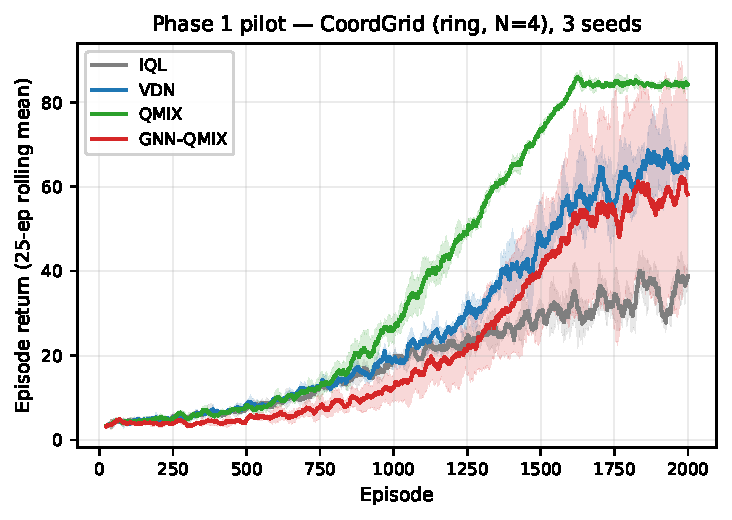
\includegraphics[width=0.5\linewidth]{figures/phase1__learning_curves.pdf}
  \caption{Phase 1 pilot learning curves on \coordgrid\ ($N=4$, ring),
  ten seeds. Shaded bands are $\pm 1$ s.d.\ across seeds of the
  25-episode rolling mean. The coordinated baselines (\vdn, \qmix) clearly
  separate from \iql, and \gnnqmix\ runs to completion, the Phase-0
  harness sanity check (Section~\ref{sec:results:pilot}).}
  \label{fig:phase1_curves}
\end{figure}

\begin{table}[h!]
  \centering
  \small
  \caption{Phase 1 final-window mean return ($N=4$, ring, 10 seeds).
  Confidence intervals are Student-$t$ 95\% across seeds; episodes-to-80\%
  is reported only for seeds that crossed the threshold within
  $5\times 10^4$ steps.}
  \label{tab:phase1_summary}
  \begin{tabular}{lrrrr}
    \toprule
    Algorithm & $n_{\text{seeds}}$ & Final mean & 95\% CI & Episodes to 80\% \\
    \midrule
    IQL & 10 & 34.62 & [32.61, 36.64] & 1375 \\
VDN & 10 & 66.023 & [62.57, 69.48] & 1528 \\
QMIX & 10 & 84.015 & [83.41, 84.62] & 1431 \\
GNN-QMIX & 10 & 66.015 & [57.11, 74.92] & 1552 \\
    \bottomrule
  \end{tabular}
\end{table}

\begin{table}[h!]
  \centering
  \small
  \caption{Phase 2 final-window mean return by condition. Edge density is
  matched between \texttt{ring} and \texttt{erdos\_renyi} by construction.}
  \label{tab:phase2_summary}
  \begin{tabular}{llrrrr}
    \toprule
    graph & $N$ & algorithm & Final mean & 95\% CI & Episodes to 80\% \\
    \midrule
    erdos\_renyi & 4 & GNN-QMIX & 7.05 & [6.29, 7.81] & 427 \\
erdos\_renyi & 4 & IQL & 34.05 & [31.99, 36.10] & 785 \\
erdos\_renyi & 4 & QMIX & 82.52 & [80.35, 84.70] & 873 \\
erdos\_renyi & 4 & VDN & 57.32 & [54.59, 60.05] & 914 \\
erdos\_renyi & 8 & GNN-QMIX & 9.18 & [8.37, 9.98] & 40 \\
erdos\_renyi & 8 & IQL & 43.26 & [40.47, 46.05] & 795 \\
erdos\_renyi & 8 & QMIX & 108.79 & [82.73, 134.84] & 961 \\
erdos\_renyi & 8 & VDN & 69.19 & [53.99, 84.39] & 969 \\
ring & 4 & GNN-QMIX & 34.76 & [24.96, 44.56] & 974 \\
ring & 4 & IQL & 28.86 & [27.10, 30.61] & 745 \\
ring & 4 & QMIX & 83.29 & [81.43, 85.15] & 876 \\
ring & 4 & VDN & 52.64 & [46.74, 58.54] & 919 \\
ring & 8 & GNN-QMIX & 19.52 & [13.88, 25.17] & 716 \\
ring & 8 & IQL & 40.10 & [34.47, 45.73] & 787 \\
ring & 8 & QMIX & 129.13 & [100.90, 157.36] & 938 \\
ring & 8 & VDN & 70.53 & [59.12, 81.94] & 908 \\
    \bottomrule
  \end{tabular}
\end{table}

\begin{table}[h!]
  \centering
  \small
  \caption{Phase 1 sanity check: IQL vs.\ each coordinated baseline on
  final-window mean return ($N=4$, ring, 10 seeds). Welch's $t$,
  Holm-corrected over the 6-pair family.}
  \label{tab:phase1_pairwise}
  \begin{tabular}{lrrr}
    \toprule
    Comparison & $\Delta$ mean return & $p_{\text{raw}}$ & $p_{\text{Holm}}$ \\
    \midrule
    IQL vs.\ VDN & 31.40 & $<0.001$ & $<0.001$ \\
IQL vs.\ QMIX & 49.39 & $<0.001$ & $<0.001$ \\
IQL vs.\ GNN-QMIX & 31.39 & $<0.001$ & $<0.001$ \\
    \bottomrule
  \end{tabular}
\end{table}

\begin{table}[h!]
  \centering
  \small
  \caption{H1 (within-condition): GNN-QMIX minus QMIX in mean final-window
  return. $p$-values are one-sided Welch $t$ ($H_a$: \gnnqmix\ $>$ \qmix),
  not corrected (single test per condition). The ordering is negative in
  every cell.}
  \label{tab:phase2_h1}
  \begin{tabular}{rlrr}
    \toprule
    $N$ & graph & $\Delta = $ GNN-QMIX $-$ QMIX & $p$ (1-sided) \\
    \midrule
    4 & erdos\_renyi & -75.47 & 1.000 \\
4 & ring & -48.54 & 1.000 \\
8 & erdos\_renyi & -99.61 & 1.000 \\
8 & ring & -109.61 & 1.000 \\
    \bottomrule
  \end{tabular}
\end{table}

\begin{table}[h!]
  \centering
  \small
  \caption{H2 (difference-of-differences): the GNN-QMIX vs.\ QMIX gap on
  ring minus the same gap on Erd\H{o}s--R\'enyi at matched edge density.
  One-sample $t$ on per-seed DiD against 0 ($H_a$: DiD $> 0$).}
  \label{tab:phase2_h2}
  \begin{tabular}{rrrrr}
    \toprule
    $N$ & $\Delta_{\text{ring}}$ & $\Delta_{\text{ER}}$ & DiD & $p$ (1-sided) \\
    \midrule
    4 & -48.54 & -75.47 & 26.93 & $<0.001$ \\
8 & -109.61 & -99.61 & -10.00 & 0.701 \\
    \bottomrule
  \end{tabular}
\end{table}

% =========================================================================
\section{Supplementary figures}
\label{app:figures}

This appendix collects the per-condition depth--diameter curves that
accompany the Phase 4 heatmap (Figure~\ref{fig:phase4_heatmap}) in the main
text.

\begin{table}[h!]
  \centering
  \small
  \caption{Phase 8 final-window return (mean over \PEseeds\ seeds) on the
  \texttt{ring} graph (the numbers behind Finding 1,
  Section~\ref{sec:results:capacity}). \mlpqmix\ is the parameter-matched
  no-graph control (identical parameter count to \gnnqmix). \emph{Capacity}
  effect $=\mlpqmix-\qmix$; \emph{graph} effect $=\gnnqmix-\mlpqmix$.}
  \label{tab:phase8}
  \begin{tabular}{lcccc}
    \toprule
    & \qmix & \mlpqmix & \gnnqmix & graph effect \\
    & {\footnotesize no cap, no graph} & {\footnotesize cap, no graph}
      & {\footnotesize cap + graph} & {\footnotesize $\gnnqmix-\mlpqmix$} \\
    \midrule
    $N=4$ & \PEqmixNfour & \PEmlpNfour & \PEgnnNfour
          & $\PEgraphGapNfour$ \;($d{=}\PEgraphDNfour$) \\
    $N=8$ & \PEqmixNeight & \PEmlpNeight & \PEgnnNeight
          & $\PEgraphGapNeight$ \;($d{=}\PEgraphDNeight$) \\
    \bottomrule
  \end{tabular}
\end{table}


\begin{figure}[h!]
  \centering
  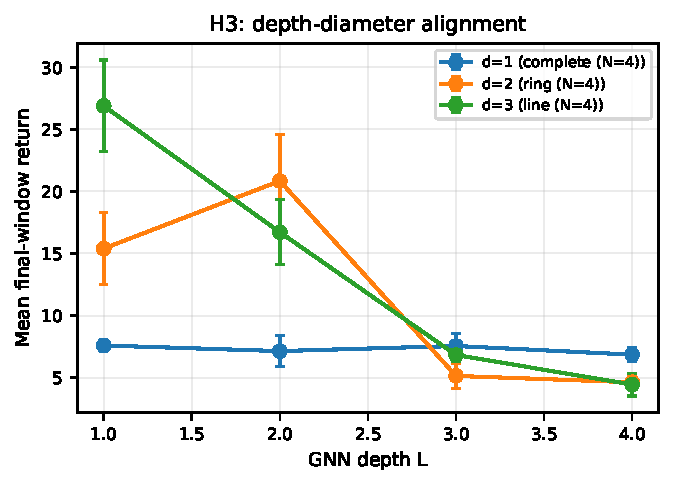
\includegraphics[width=0.62\textwidth]{figures/phase4__depth_diameter_curves.pdf}
  \caption{Phase 4 depth--diameter curves (companion to the heatmap in
  Section~\ref{sec:results:ablation}). Final-window return vs.\ GCN depth
  $L$ for each graph diameter $d$; the over-depth cliff at $L\ge 3$ is
  visible on every diameter.}
  \label{fig:phase4curves}
\end{figure}


%% =========================================================================
\section{Reproducibility Checklist for JAIR}
Select the answers that apply to this research -- one per item.

\subsection*{All articles:}
\begin{enumerate}
  \item All claims investigated in this work are clearly stated. \textbf{[yes]}
  \item Clear explanations are given how the work reported substantiates the claims. \textbf{[yes]}
  \item Limitations or technical assumptions are stated clearly and explicitly. \textbf{[yes]}
  \item Conceptual outlines and/or pseudo-code descriptions of the AI methods introduced in this work are provided, and important implementation details are discussed. \textbf{[yes]}
  \item Motivation is provided for all design choices, including algorithms, implementation choices, parameters, data sets and experimental protocols beyond metrics. \textbf{[yes]}
\end{enumerate}

\subsection*{Articles containing theoretical contributions:}
Does this paper make theoretical contributions? \textbf{[no]}

\subsection*{Articles reporting on computational experiments:}
Does this paper include computational experiments? \textbf{[yes]}
\begin{enumerate}
  \item All source code required for conducting experiments is included in an online appendix or will be made publicly available upon publication of the paper. The online appendix follows best practices for source code readability and documentation as well as for long-term accessibility. \textbf{[yes]}
  \item The source code comes with a license that allows free usage for reproducibility purposes. \textbf{[yes]}
  \item The source code comes with a license that allows free usage for research purposes in general. \textbf{[yes]}
  \item Raw, unaggregated data from all experiments is included in an online appendix or will be made publicly available upon publication of the paper. The online appendix follows best practices for long-term accessibility. \textbf{[yes]}
  \item The unaggregated data comes with a license that allows free usage for reproducibility purposes. \textbf{[yes]}
  \item The unaggregated data comes with a license that allows free usage for research purposes in general. \textbf{[yes]}
  \item If an algorithm depends on randomness, then the method used for generating random numbers and for setting seeds is described in a way sufficient to allow replication of results. \textbf{[yes]}
  \item The execution environment for experiments, the computing infrastructure (hardware and software) used for running them, is described, including GPU/CPU makes and models; amount of memory (cache and RAM); make and version of operating system; names and versions of relevant software libraries and frameworks. \textbf{[yes]}
  \item The evaluation metrics used in experiments are clearly explained and their choice is explicitly motivated. \textbf{[yes]}
  \item The number of algorithm runs used to compute each result is reported. \textbf{[yes]}
  \item Reported results have not been ``cherry-picked'' by silently ignoring unsuccessful or unsatisfactory experiments. \textbf{[yes]}
  \item Analysis of results goes beyond single-dimensional summaries of performance (e.g., average, median) to include measures of variation, confidence, or other distributional information. \textbf{[yes]}
  \item All (hyper-) parameter settings for the algorithms/methods used in experiments have been reported, along with the rationale or method for determining them. \textbf{[yes]}
  \item The number and range of (hyper-) parameter settings explored prior to conducting final experiments have been indicated, along with the effort spent on (hyper-) parameter optimisation. \textbf{[partially]}
  \item Appropriately chosen statistical hypothesis tests are used to establish statistical significance in the presence of noise effects. \textbf{[yes]}
\end{enumerate}

\subsection*{Articles using data sets:}
Does this work rely on one or more data sets (possibly obtained from a benchmark generator or similar software artifact)? \textbf{[yes]}
\begin{enumerate}
  \item All newly introduced data sets are included in an online appendix or will be made publicly available upon publication of the paper. The online appendix follows best practices for long-term accessibility with a license that allows free usage for research purposes. \textbf{[yes]}
  \item The newly introduced data set comes with a license that allows free usage for reproducibility purposes. \textbf{[yes]}
  \item The newly introduced data set comes with a license that allows free usage for research purposes in general. \textbf{[yes]}
  \item All data sets drawn from the literature or other public sources (potentially including authors' own previously published work) are accompanied by appropriate citations. \textbf{[yes]}
  \item All data sets drawn from the existing literature (potentially including authors' own previously published work) are publicly available. \textbf{[yes]}
  \item All new data sets and data sets that are not publicly available are described in detail, including relevant statistics, the data collection process and annotation process if relevant. \textbf{[yes]}
  \item All methods used for preprocessing, augmenting, batching or splitting data sets (e.g., in the context of hold-out or cross-validation) are described in detail. \textbf{[NA]}
\end{enumerate}

\subsection*{Explanations on any of the answers above (optional):}
All environments (the \coordgrid\ gridworld and the \tokenmatch\ referential game) are
procedural generators released with the code (MIT-licensed); the external MPE and LBF
tasks are cited and publicly available. Hyper-parameters were pre-registered and locked
before confirmatory runs, so per-experiment tuning effort was deliberately minimal.

\end{document}
